%%
%% This is file `sample-sigplan.tex',
%% generated with the docstrip utility.
%%
%% The original source files were:
%%
%% samples.dtx  (with options: `sigplan')
%% 
%% IMPORTANT NOTICE:
%% 
%% For the copyright see the source file.
%% 
%% Any modified versions of this file must be renamed
%% with new filenames distinct from sample-sigplan.tex.
%% 
%% For distribution of the original source see the terms
%% for copying and modification in the file samples.dtx.
%% 
%% This generated file may be distributed as long as the
%% original source files, as listed above, are part of the
%% same distribution. (The sources need not necessarily be
%% in the same archive or directory.)
%%
%% The first command in your LaTeX source must be the \documentclass command.
\documentclass[sigconf,review,anonymous]{acmart}
\settopmatter{printfolios=true,printccs=false,printacmref=false}

%%
%% \BibTeX command to typeset BibTeX logo in the docs
\AtBeginDocument{%
  \providecommand\BibTeX{{%
    \normalfont B\kern-0.5em{\scshape i\kern-0.25em b}\kern-0.8em\TeX}}}

%% Rights management information.  This information is sent to you
%% when you complete the rights form.  These commands have SAMPLE
%% values in them; it is your responsibility as an author to replace
%% the commands and values with those provided to you when you
%% complete the rights form.
% \setcopyright{acmcopyright}
% \copyrightyear{2018}
% \acmYear{2018}
% \acmDOI{10.1145/1122445.1122456}

%% These commands are for a PROCEEDINGS abstract or paper.
% \acmConference[Woodstock '18]{Woodstock '18: ACM Symposium on Neural
%   Gaze Detection}{June 03--05, 2018}{Woodstock, NY}
% \acmBooktitle{Woodstock '18: ACM Symposium on Neural Gaze Detection,
%   June 03--05, 2018, Woodstock, NY}
% \acmPrice{15.00}
% \acmISBN{978-1-4503-9999-9/18/06}
\acmConference[ESEC/FSE 2021]{The 29th ACM Joint European Software Engineering Conference and Symposium on the Foundations of Software Engineering}{23 - 27 August, 2021}{Athens, Greece}


%%
%% Submission ID.
%% Use this when submitting an article to a sponsored event. You'll
%% receive a unique submission ID from the organizers
%% of the event, and this ID should be used as the parameter to this command.
%%\acmSubmissionID{123-A56-BU3}

%%
%% The majority of ACM publications use numbered citations and
%% references.  The command \citestyle{authoryear} switches to the
%% "author year" style.
%%
%% If you are preparing content for an event
%% sponsored by ACM SIGGRAPH, you must use the "author year" style of
%% citations and references.
%% Uncommenting
%% the next command will enable that style.
%%\citestyle{acmauthoryear}


% tables
\usepackage{tabularx}
\usepackage{booktabs}
\usepackage{algorithm}
\usepackage[noend]{algpseudocode}

% xspace command
\usepackage{xspace}

% From https://tex.stackexchange.com/questions/177025/
\makeatletter
\newcounter{algorithmicH}% New algorithmic-like hyperref counter
\let\oldalgorithmic\algorithmic
\renewcommand{\algorithmic}{%
  \stepcounter{algorithmicH}% Step counter
  \oldalgorithmic}% Do what was always done with algorithmic environment
\renewcommand{\theHALG@line}{ALG@line.\thealgorithmicH.\arabic{ALG@line}}
\makeatother

% lstlisting command
\usepackage{listings}
\usepackage[scaled]{beramono}
\newcommand*\LSTfont{\Small\fontencoding{T1}\ttfamily\SetTracking{encoding=*}{-60}\lsstyle}
\lstset{language=Java,
  frame=none,
  aboveskip=1.5pt,
  belowskip=0pt,
  showstringspaces=false,
  columns=flexible,
  basicstyle=\LSTfont,
  numbers=none,
  numberstyle=\tiny\color{black},
  keywordstyle=\color{black},
  commentstyle=\color{black},
  stringstyle=\color{black},
  breaklines=true,
  breakatwhitespace=true,
  tabsize=3,
  %emph={@NonNegative,@Positive,@GTENegativeOne,@LTLengthOf,@LTEqLengthOf,@IndexFor,@IndexOrHigh,@IndexOrLow,@HasSubsequence,@LessThan,@SameLen,@SearchIndexFor,@MinLen,@ArrayLen,@IntVal,@IntRange,@LengthOf,@UpperBoundUnknown,@LowerBoundUnknown,int,double,List,Map,Object,SerialDate,Long,Integer,DefaultPolarItemRenderer,LegendItem,PolarPlot,XYDataset,long,T,String,string,byte,InputStream,CategoryDataset,DatasetRenderingOrder,ArrayList,Entry,Values,Number,ValuesContract,ImmutableIntArray,Dataset,XYZDataset}, emphstyle=\color{blue}
}

% Graphics
\usepackage{tikz}
\usetikzlibrary{arrows,automata,positioning}

% Change font and line spacing for figure captions
\usepackage{setspace,caption}
\captionsetup{labelfont={small,bf}, textfont={small,bf,stretch=0.8}, labelsep=colon, margin=0pt}

\usepackage{flushend} % balanced columns on last page

% cref command; best to load last
\usepackage{cleveref}
\newcommand{\crefrangeconjunction}{--}

%%
%% end of the preamble, start of the body of the document source.
\begin{document}

%%% Todo comments
%% Comment out one of these two definitions.
%\newcommand{\todo}[1]{\relax}
\newcommand{\todo}[1]{{\color{red}\bfseries [[#1]]}}
\newcommand{\manu}[1]{\todo{#1 --MS}}

% Don't show todo commands if this macro is defined.
\ifdefined\notodocomments
  \renewcommand{\todo}[1]{\relax}
\fi

\newif\ifanonymous
\anonymoustrue

\newcommand{\anonurl}[1]{\ifanonymous URL removed for anonymity.\else\url{#1}\fi}
\newcommand{\footnoteanonurl}[1]{\footnote{\anonurl{#1}}}

%% The anonymized name of the tool
%% TODO: come up with a better name.
\newcommand{\toolanon}{Plumber\xspace}
%% The name of the tool to use
\newcommand{\Tool}{\toolanon}
%% TODO: remove this.  (The tool name is capitalized and the LaTeX source
%% reads best when the macro is also capitalized.)
\newcommand{\tool}{\toolanon}

% \|name| or \mathid{name} denotes identifiers and slots in formulas
\def\|#1|{\mathid{#1}}
\newcommand{\mathid}[1]{\ensuremath{\mathit{#1}}}
% \<name> or \codeid{name} denotes computer code identifiers
\def\<#1>{\codeid{#1}}
% \protected\def\codeid#1{\ifmmode{\mbox{\sf{#1}}}\else{\sf #1}\fi}
% \protected\def\codeid#1{\ifmmode{\mbox{\ttfamily{#1}}}\else{\ttfamily #1}\fi}
\protected\def\codeid#1{\ifmmode{\mbox{\smaller\ttfamily{#1}}}\else{\smaller\ttfamily #1}\fi}

\newcommand{\CalledMethodsBottom}{\<@Call\-ed\-Meth\-ods\-Bottom>\xspace}
\newcommand{\EnsuresCalledMethods}{\<@En\-sures\-Call\-ed\-Meth\-ods>\xspace}
\newcommand{\MustCall}{\codeid{@Must\-Call}\xspace}
\newcommand{\MustCallAlias}{\codeid{@Must\-Call\-Alias}\xspace}
\newcommand{\MustCallUnknown}{\codeid{@Must\-Call\-Unknown}\xspace}
\newcommand{\ResetMustCall}{\<@Reset\-Must\-Call>\xspace}

% "trule" stands for ``type rule''
\newcommand{\trule}[2]{\[\frac{#1}{#2}\]}
\newcommand{\truleinline}[2]{\ensuremath{#1\mathrel{\vdash}#2}}
\newcommand{\hastype}[1]{\mathbin{:}\trtext{#1}}
\newcommand{\trcode}[1]{\codeid{\smaller\smaller #1}}
\newcommand{\trtext}[1]{\mbox{\smaller\smaller #1}}
\newcommand{\trquoted}[1]{\trcode{"}#1\trcode{"}}


\hyphenation{type-state}        % LaTeX defaults to "types-tate"

% Reduce indentation in lists.
\setlength{\leftmargini}{.75\leftmargini}
\setlength{\leftmarginii}{.75\leftmarginii}
\setlength{\leftmarginiii}{.75\leftmarginiii}

\newcommand{\prefigcaption}{\vspace{-10pt}}
\newcommand{\posttablecaption}{\vspace{-10pt}}


%%
%% The "title" command has an optional parameter,
%% allowing the author to define a "short title" to be used in page headers.
\title{Lightweight and Modular Resource Leak Verification}

%%
%% The "author" command and its associated commands are used to define
%% the authors and their affiliations.
%% Of note is the shared affiliation of the first two authors, and the
%% "authornote" and "authornotemark" commands
%% used to denote shared contribution to the research.


%%
%% By default, the full list of authors will be used in the page
%% headers. Often, this list is too long, and will overlap
%% other information printed in the page headers. This command allows
%% the author to define a more concise list
%% of authors' names for this purpose.
%\renewcommand{\shortauthors}{Trovato and Tobin, et al.}

%%
%% The abstract is a short summary of the work to be presented in the
%% article.
\begin{abstract}
  A resource leak occurs when a program allocates a resource, such as a
  socket or file handle, but fails to deallocate
  it.  Resource leaks are an important, common problem that cause resource
  starvation, slowdowns, and crashes.  Previous techniques
  to prevent resource leaks are unsound,
  imprecise, inapplicable to existing code, slow, or a combination
  of these.\looseness=-1
  
  We observe that detecting a resource leak for a variable involves three
  parts: 1) tracking its \emph{must-call obligations},
  2) tracking which methods have been called on it, and 3) comparing
  the results of these to check if its obligations have been fulfilled.
  Our key insight is that these can be reduced to an
  accumulation problem, a class of typestate problems amenable
  to sound and modular checking without the need for a heavyweight,
  whole-program alias analysis.  We developed a
  baseline leak checker via this approach.
  % Rashmi said the following was too negative, and I agree:
  % , but found
  % that it suffered from an excess of false positives.
  The precision of an accumulation analysis can be improved by computing
  targeted aliasing information, and we devised three novel techniques
  that use this capability to achieve precision in practice:
  a lightweight ownership transfer system;
  a specialized resource alias analysis;
  and a system
  to create a fresh obligation when a non-final resource field
  is updated.
  % check that re-assignments to non-final fields
  % that hold a resource are safe.
  %% MK: the below is too wordy - less jargon in the abstract, just the summary
  %%
  %% Lightweight ownership tracking is a
  %% technique to help determine which alias is responsible for releasing
  %% a resource.  Since our goal is only to prevent resource leaks, our
  %% ownership tracking avoids many of the heavyweight aliasing
  %% restrictions associated with other ownership type systems.
  %% Resouce alias analysis is a specialized, lightweight must-alias analysis
  %% that identifies program elements that definitely control the same resource.
  %% Accumulation frames extend the theory of accumulation analysis to permit
  %% certain kinds of cycles in the typestate automaton.

  Our approach occupies a unique slice of the design space when compared
  to prior approaches: it is sound
  and runs quickly compared to heavier-weight
  \todo{mention ``unsound''?}
  approaches (running in minutes on programs that a
  state-of-the-art approach
  took hours to analyze).
  We implemented our techniques for Java in an open-source tool
  called \Tool.
  \Tool revealed 45 real bugs in widely-deployed software.
  It scales well, has a manageable false positive rate
  (\todo{similar to the resource leak analysis built into the Eclipse IDE}), and
  imposes only a small additional annotation burden (1/2000 LoC) for developers.
\end{abstract}

%%
%% The code below is generated by the tool at http://dl.acm.org/ccs.cfm.
%% Please copy and paste the code instead of the example below.
%%
% \begin{CCSXML}
% <ccs2012>
%  <concept>
%   <concept_id>10010520.10010553.10010562</concept_id>
%   <concept_desc>Computer systems organization~Embedded systems</concept_desc>
%   <concept_significance>500</concept_significance>
%  </concept>
%  <concept>
%   <concept_id>10010520.10010575.10010755</concept_id>
%   <concept_desc>Computer systems organization~Redundancy</concept_desc>
%   <concept_significance>300</concept_significance>
%  </concept>
%  <concept>
%   <concept_id>10010520.10010553.10010554</concept_id>
%   <concept_desc>Computer systems organization~Robotics</concept_desc>
%   <concept_significance>100</concept_significance>
%  </concept>
%  <concept>
%   <concept_id>10003033.10003083.10003095</concept_id>
%   <concept_desc>Networks~Network reliability</concept_desc>
%   <concept_significance>100</concept_significance>
%  </concept>
% </ccs2012>
% \end{CCSXML}

% \ccsdesc[500]{Computer systems organization~Embedded systems}
% \ccsdesc[300]{Computer systems organization~Redundancy}
% \ccsdesc{Computer systems organization~Robotics}
% \ccsdesc[100]{Networks~Network reliability}

%%
%% Keywords. The author(s) should pick words that accurately describe
%% the work being presented. Separate the keywords with commas.
% \keywords{datasets, neural networks, gaze detection, text tagging}

%% A "teaser" image appears between the author and affiliation
%% information and the body of the document, and typically spans the
%% page.
%% \begin{teaserfigure}
%%   \includegraphics[width=\textwidth]{sampleteaser}
%%   \caption{Seattle Mariners at Spring Training, 2010.}
%%   \Description{Enjoying the baseball game from the third-base
%%   seats. Ichiro Suzuki preparing to bat.}
%%   \label{fig:teaser}
%% \end{teaserfigure}

%%
%% This command processes the author and affiliation and title
%% information and builds the first part of the formatted document.
\maketitle

\section{Introduction}
\label{sec:intro}

%% Resource leaks are a classic problem, and extant approaches to preventing
%% them are either too expensive or unsound.

A resource leak occurs when some finite resource managed by the
programmer is not explicitly disposed of. In an unmanaged language
like C, that explicit resource might be memory; in a managed language
like Java, it might be a file descriptor, a socket, or a database
connection.  Resource leaks continue to cause severe failures, even in
modern, heavily-used Java applications~\cite{ghanavati2020memory}.
This state-of-the-practice does not differ much from two decades
ago~\cite{WeimerN04}.
Microsoft engineers consider resource leaks to be one of the most
significant development challenges~\cite{LoNZ2015}.
% The fact that
% resource leaks remain such a serious problem despite decades of
% research and improvements in languages and tooling shows that
Preventing resource leaks remains an urgent, difficult, open problem.

%% An ideal tool for preventing resource leaks would be fast, sound, and precise.

Ideally, a tool for preventing resource leaks would be:
\vspace{-5pt}
\begin{itemize}
\item \emph{applicable} to
  % leakable resources in
  existing code with few code changes,
\item \emph{sound}, so that undetected resource leaks do not slip into
  the program;
\item \emph{precise}, so that developers are not bothered by excessive false positive
  warnings; and
\item \emph{fast}, so that it scales to real-world programs and
  developers can use it regularly.
\end{itemize}
\vspace{-5pt}

%% Extant approaches fail at least one of these: bug finders like the analysis
%% in ecj are unsound; complex analyses based on typestate are either too slow
%% (cite the Eurosys 2019 paper on Grapple, with numbers on run time), unsound, or both.
\noindent
Extant approaches fail at least one of these criteria.
Language-based features may not apply to all uses of resource variables:
Java's try-with-resources statement~\cite{try-with-resources}, for example, can
only close resource types that implement the \<java.lang.AutoCloseable> interface,
and cannot handle
common resource usage patterns that span multiple procedures. 
Heuristic bug-finding tools for leaks, such as those built into Java IDEs including
Eclipse~\cite{ecj-resource-leak} and IntelliJ
IDEA~\cite{idea-resource-leak}, 
are fast and applicable to legacy
code, but they are unsound.
%% They are equally as imprecise as our tool, so don't bad-mouth them.
% and can be highly imprecise (\cref{sec:compare}).
Inter-procedural typestate or dataflow analyses~\cite{TorlakC10,zuo2019grapple}
achieve more precise
%% In our experiments, they found fewer defects, and we didn't compare complexity.
% results---and can find more complex defects than bug-finders,
results---though they usually remain unsound---but
their whole-program analysis can require hours to analyze a large-scale Java program.
Finally, ownership type
systems~\cite{clarke2013ownership} as employed in languages like
Rust~\cite{klabnik2018rust} can prevent nearly all resource leaks (see
\cref{sec:rw-language}), but using them would require a significant rewrite for
a legacy codebase, a substantial task which is often infeasible.
% require
% significantly rewriting the program, 
% and prevents them from being applicable to legacy codebases and coding styles.

The goal of a leak detector for a Java-like language is to ensure that required
methods (such as \<close()>) are called on all relevant objects; we deem this
a \emph{must-call} property.  Verifying a must-call property requires
checking that required methods (or \emph{must-call obligations}) have been
called at any point where an object may become unreachable.  A static
verifier does this by computing an
under-approximation of invoked methods.  Our key insight is that checking of
must-call properties is an \emph{accumulation problem}, and hence does not
require heavyweight whole-program analysis. Our contribution is a resource leak
verifier that leverages this insight to satisfy all four requirements: it is
applicable, sound, precise, and fast.\looseness=-1

An accumulation analysis~\cite{KelloggRSSE2020}
is a special-case of typestate analysis~\cite{StromY86}.
Typestate analysis attaches a finite-state machine (FSM)
to each program element of a given type, and transitions the state of the
FSM whenever a relevant operation is performed.
In an accumulation analysis,
the order of operations performed cannot change what is subsequently
permitted, and executing more operations cannot add additional
restrictions.  Unlike arbitrary typestate analyses, accumulation analyses can
be build in a sound, modular fashion without \emph{any} whole-program alias
analysis, improving scalability and usability.

Recent work~\cite{KelloggRSSE2020} presented an accumulation analysis for
verifying that certain methods are invoked on each object
before a specific call (e.g., \<build()>).
Resource leak checking is similar in that certain methods must be invoked
on each object before it becomes unreachable.
An object becomes unreachable when its references go out
of scope or are overwritten.
By making an analogy between object-unreachability points and
method calls, we show that resource leak checking is an accumulation
problem and hence is amenable to sound, modular, and lightweight analysis.

%% Old version of the above paragraph.
% Recent work~\cite{KelloggRSSE2020} presented an accumulation analysis for
% verifying that certain methods are invoked on each object reference
% before a specific call (e.g., \<build()>).
% Conceptually,
% we can build a resource leak verifier by extending this technique
% to check that required methods are invoked before a reference goes out
% of scope or is overwritten, either of which could cause an object to become unreachable.
% This reduction of possible object-unreachability points to
% method calls shows
% that resource leak checking is an accumulation
% problem and hence is amenable to sound, modular, and lightweight analysis.

There are two key challenges for this leak-checking approach.  First,
due to subtyping, the declared type of a reference may not accurately represent
its must-call obligations; we devised a simple type system to soundly capture
these obligations.  Second, the approach is sound, but highly imprecise (more so than in
previous work~\cite{KelloggRSSE2020}) without targeted reasoning about
aliasing.  The most important patterns to
handle are:
\begin{itemize}
\item copying of resources via parameters and returns, or storing of resources in
final fields (the RAII pattern~\cite{raii});
\item wrapper types, which share their must-call obligations with one of their fields; and,
\item storing resources in non-final fields, which might be lazily initialized or
  written more than once.
\end{itemize}
To address this need,
we introduced an intra-procedural
dataflow analysis for alias tracking, and extended it with three sound
techniques to improve precision:
\begin{itemize}
\item a lightweight ownership transfer system. This system
  indicates which reference is responsible for resolving a must-call
  obligation. Unlike typical ownership type systems, our approach does
  not impact the privileges of non-owning references.
\item resource aliasing, for cases
  %% "in which" is better English, but "when" saves a line.
  % in which
  when
  a resource's must-call obligations
  can be resolved by closing one of multiple references.
\item a system for creating new obligations at locations other than the
  constructor, which allows our system to handle lazy initialization or re-initialization.
\end{itemize}
Variants of some of these ideas exist in previous work.  We bring
them together in a general, modular manner, with full verification and
the ability for programmers to easily extend checking to their own
types and must-call properties.
%
Our approach occupies a novel point in the design space for a leak detector:
unlike most prior work, it is sound; it is an order of magnitude faster than
state-of-the-art whole-program analyses; it has a false positive rate similar
to a state-of-the-practice heuristic bug-finder; and, though it does require manual
annotations from the programmer, its annotation burden is reasonable: about
1 annotation for every 1,500 lines of non-comment, non-blank code. 

Our contributions are:
\begin{itemize}
\item the insight that the resource leak problem is an accumulation
  problem, and
  % a novel set of
  an analysis approach based on
  this fact (\cref{sec:base-type-systems}).
\item three
  % novel
  innovations that improve the precision of our analysis via targeted reasoning about aliasing:
  a lightweight ownership transfer system
  (\cref{sec:lightweight-ownership}), a lightweight resource-alias
  tracking analysis (\cref{sec:must-call-choice}), and a system for
  handling lazy or multiple initialization (\cref{sec:reset-must-call}).
\item an open-source implementation for Java,
  called \tool (\cref{sec:implementation}).
\item an empirical evaluation: case studies on heavily-used
  Java programs (\cref{sec:case-studies}),
  an ablation study that shows the contributions of each innovation to
  \tool's precision (\cref{sec:ablation}), and a comparison to
  other state-of-the-art approaches that demonstrates the unique strengths
  of our approach (\cref{sec:compare}).
%% \item a comparison to alternative approaches to resource leak
%%   checking, that demonstrates that our approach occupies a unique
%%   point in the design space: faster and more usable than heavy-weight
%%   typestate systems, but sound and able to find even subtle bugs,
%%   unlike heuristic bug-finders (\cref{sec:compare}).
\end{itemize}
  

% LocalWords:  unmanaged leakable finalizers RAII


% the technical sections about the core accumulation systems: called methods,
% must-call, and the must call invoked worklist algorithm.

\section{Leak detection via accumulation}
\label{sec:base-type-systems}

This section presents a sound, modular, accumulation-based
resource leak checker (``\tool'').
\Cref{sec:lightweight-ownership,sec:reset-must-call,sec:must-call-choice}
soundly enhance its precision.

\Tool is composed of three cooperating analyses:
\begin{enumerate}
\item a taint tracking type system (\cref{sec:must-call}) computes a conservative
  \emph{overapproximation} of the set of methods that might need to be called
  on each expression in the program.
\item an accumulation type system (\cref{sec:called-methods}) computes
  a conservative \emph{underapproximation} of the set of methods that are
  actually called on each expression in the program.
\item a dataflow analysis (\cref{sec:must-call-invoked}) checks consistency of the results of the two
  above-mentioned type systems and provides a platform for targeted alias reasoning.  It issues an error if some
  method that might need to be called on an expression is not always invoked before the
  expression goes out of scope or is overwritten.
\end{enumerate}

% \noindent
% This section uses \cref{fig:example} as a motivating example.
% It shows
% a safe use of a \<Socket>---a resource that must be closed before
% it is deallocated.


\subsection{Background on Pluggable Types}
\label{sec:background}

\Cref{sec:must-call,sec:called-methods} describe
\emph{pluggable type systems}~\cite{FosterFFA99}
that are layered on top of the type system of the host
language.  Types in a pluggable type system are composed of two parts:
a \emph{type qualifier} and a base type. The type qualifier is the
part of the type that is unique to the pluggable type system; the base
type is a type from the host language. Our implementation is for Java
(see \cref{sec:implementation}), so we use the Java syntax for type
qualifiers: ``\<@>'' before a type indicates that it is a type
qualifier, and a type without ``\<@>'' is a base type.
This paper sometimes omits the base type when it is obvious from context.\looseness=-1

A type system checks programmer-written types.  Our system requires the
programmer to write types on method signatures, but within method bodies it
uses flow-sensitive type refinement, a dataflow analysis that performs type
inference.  This permits an expression to have different types on different
lines of the program.


\begin{figure}
  \lstinputlisting{simplesocket.txt}
  \prefigcaption
  \caption{A safe use of a \<Socket> resource.}
  \label{fig:example}
\end{figure}

\subsection{A Type System for Must-Call Obligations}
\label{sec:must-call}

\begin{figure}

\begin{tikzpicture}[->, shorten >= 1pt, auto, node distance=0.3cm]
  \tikzstyle{every state}=[fill=none,draw=none,text=black, minimum size = 0.5cm, shape = rectangle]
  
  \node[state]        (TOP)                                   {\parbox{4cm}  {\centering \small \<@MustCallUnknown> $= \top$}};
  \node[state]         (MCAB)      [below   = of TOP]        {\parbox{4cm}  {\centering \small \<@MustCall(\{"a", "b"\})>}};
  \node[state]         (MCA)    [below  = of MCAB, xshift=-2.2cm]         {\parbox{4cm} {\centering \small \<@MustCall(\{"a"\})>}};
  \node[state]         (MCB)    [below  = of MCAB, xshift=2.2cm]         {\parbox{4cm} {\centering \small \<@MustCall(\{"b"\})>}};
  \node[state]         (BOT)     [below      = of MCAB, yshift=-0.8cm]       {\parbox{4cm}  {\centering \small \<@MustCall(\{\})> $= \bot$}};

  \path

  (MCAB)        edge        node {} (TOP)
  
  (MCA)         edge        node {} (MCAB)
  (MCB)         edge        node {} (MCAB)
  
  (BOT)         edge        node {} (MCA)
  (BOT)         edge        node {} (MCB)

  ;

\end{tikzpicture}
% \prefigcaption
\caption{Part of the \<MustCall> type hierarchy for representing which methods must be
  called; the full hierarchy is a
  lattice of arbitrary size.
  If an expression's type has qualifier \<@Must\-Call(\{"a", "b"\})>, then
  the methods ``\<a>'' and ``\<b>'' might need to be called before the
  expression is deallocated.
  Arrows represent
  subtyping relationships.
}
\label{fig:must-call-hierarchy}
\end{figure}

The Must Call type system tracks which methods might need to be called
on a given expression.  This type system---and
our entire analysis---is not specific to resource leaks. Another such
  property is that the
  \<build()> method of a builder~\cite{designpatterns} should always
  be called.

The Must Call type system supports two qualifiers: \MustCall and
\MustCallUnknown. The \MustCall qualifier's arguments are the
methods that
% "the annotated value" is inaccurate (it is accurate to say "the value of the
% expression with that annotated type"), but is probably clear enough.
the annotated value
must call. The declaration
\MustCall\<(\{"a"\}) Object obj> means that before \<obj> is
deallocated, \<obj.a()> might need to be called.
\Tool conservatively requires all these methods to be called,
and it issues a warning if they are not.

For example, consider \cref{fig:example}. The expression \<null> has type
\MustCall\<(\{\})>---it has no obligations
to call particular methods---so \<s> has that type after its initialization.
The \<new> expression has type \MustCall\<("close")>, and therefore
\<s> has that type after the assignment.
At the start of the \<finally> block, where both values for \<s> flow,
the type of \<s> is their least upper bound, which is \MustCall\<("close")>.

% Note that the type \MustCall\<("close")>
% can represent anything that \emph{might} need to
% call \<close()>: for example, at the entrance to
% the \<finally> block in \cref{fig:example}, \<s>'s
% actual value might either be \<null>, which does not
% need to call any methods, or an open \<Socket>, which does.
% Thus, either the obligation to close or no obligation at all
% can be represented by the static
% type \MustCall\<(\{"close"\}) Socket>, which can be read as ``a
% Socket that might need to call close before it is deallocated''.

Part of the type hierarchy appears in \cref{fig:must-call-hierarchy}.
All types are subtypes of \MustCallUnknown.
The subtyping relationship for \MustCall type qualifiers is:
\trule{A \subseteq B}{\MustCall\<(A)> \sqsubseteq \MustCall\<(B)>}
The default type qualifier is \MustCall\<(\{\})> for base types without a
programmer-written type qualifier.\footnote{For unannotated local variable types,
  flow-sensitive type refinement infers a qualifier.}
% By writing another type qualifier on the declaration of a class, a
% user can specify a different default for raw types of that class.
Our implementation
provides JDK annotations which require that every 
object of \<Closeable> type must have the \<close()> method called before
it is deallocated, with exceptions for types that do not have an underlying
resource, e.g., \<ByteArrayOutputStream>.

% also provides an ``inheritable'' version of the \MustCall annotation,
% which allows us to annotate a class (or interface) and all of its subtypes.
% For example, we use such an annotation on \<java.io.Closeable> to indicate
% that all \<Closeable> objects must have the \<close()> method called before
% they are deallocated.

%% This is redundant, I think.
% A benefit of using a type system for tracking must-call obligations is
% that \tool can use local type inference to refine the obligations of
% a particular variable. For example, if the only assignment to \<s>
% in \cref{fig:example} were the initial assignment to \<null>, then
% \tool would be able to determine that \<s> does not have a must-call
% obligation.


\subsection{A Type System for Called Methods}
\label{sec:called-methods}

% \todo{Mike changed ``our types system for inferring'' to ``our type system
%   tracks''.  Let's lay off use of ``infer'' because it implies we have
%   written a type inference tool, when what we have really written is a
%   type-checking tool (with local type inference).}

\begin{algorithm}[t]
  \caption{Finding unfulfilled \MustCall obligations in a method.
    \Cref{alg:helpers} defines helper functions.
  }
  \label{alg:consistency-checker}
  \begin{algorithmic}[1]
  \Procedure{FindMissedCalls}{$CFG$}
  \State \textit{// D maps each statement s to a set of dataflow facts reaching}
  \State \textit{// s.  Each fact is of the form $\langle P, e \rangle$, where P is a set of variables}
  \State \textit{// that must-alias e and e is an expression with a nonempty}
  \State \textit{// must-call obligation.}
  \State $D \gets \textsc{InitialObligations}(CFG)$ \label{li:call-initial-obs}
  \While{$D$ has not reached fixed point}
    \For{$s \in \mathit{CFG.statements}$, $\langle P, e \rangle \in D(s)$}
    \If{$s$ is $\mathit{exit}$} \label{li:end-scope}
      \State report a must-call violation for $e$
    \ElsIf{$\neg \textsc{MCSatisfiedAfter}(P,s)$} \label{li:check-satisfied}
%    \State // \textit{propagate to successors}
    \State $kill \gets $ $s$ assigns a variable ? $\{s.LHS\}$ : $\emptyset$ \label{li:compute-kill}
    \State $gen \gets \textsc{CreatesAlias}(P,s)$ ? $\{s.LHS\}$ : $\emptyset$ \label{li:compute-gen} 
    % \If{$s$ is \lstinline{p = q} and $q \in P$}
    % \State $gen \gets \{p\}$
    % \EndIf
    \State $N \gets (P - kill) \cup gen$ \label{li:compute-new-mc-aliases}
 %   \State // \textit{we even propagate }$\emptyset$\textit{; error reported at exit}
    \State $\forall t \in \mathit{CFG.succ}(s)\ .\ D(t) \leftarrow D(t) \cup \lbrace \langle
    N, e \rangle \rbrace$ \label{li:prop-to-succs}
    \EndIf
    \EndFor
  \EndWhile \label{li:alg-loop-end}
  \EndProcedure
  \Procedure{InitialObligations}{$CFG$}
  \State $D \gets \{ s \mapsto \emptyset\ |\ s \in \mathit{CFG.statements} \}$\label{li:start-init}
  \For{$p \in \mathit{CFG.formals}$, $t \in \mathit{CFG.succ}(\mathit{CFG.entry})$}\label{li:init-formals}
    \If{$\textsc{HasObligation}(p)$}
      \State $D(t) \gets D(t) \cup \lbrace \langle \{p\}, p \rangle \rbrace$
    \EndIf
  \EndFor \label{li:end-init-formals}
  \For{$s \in \mathit{CFG.statements}$ of the form \lstinline{p = m(p1, p2, ...)}} \label{li:init-calls}
    \State $\forall t \in \mathit{CFG.succ}(s)\ .\ D(t) \leftarrow D(t) \cup \textsc{FactsFromCall}(s)$
  \EndFor  \label{li:end-init}
  \State \Return $D$
  \EndProcedure
  \end{algorithmic}
\end{algorithm}


\begin{algorithm}[h]
  \caption{Helper functions for \cref{alg:consistency-checker}.  Except for
  \textsc{MCAfter} and \textsc{CMAfter}, all functions will be replaced with
  more sophisticated versions in
  \cref{sec:lightweight-ownership,sec:must-call-choice,sec:reset-must-call}.
  \todo{Ensure the two algorithms appear on the same page.}
}
  \label{alg:helpers}
  \begin{algorithmic}[1]
  \State // \textit{Does e introduce a must-call obligation to check?}
  \Procedure{HasObligation}{$e$}
  \State \Return $e$ has a declared \MustCall type
  \EndProcedure
  \State // \textit{s must be a call statement p = m(p1, p2, ...)}
  \Procedure{FactsFromCall}{$s$}
  \State $p \gets s.LHS, c \gets s.RHS$
  \State \Return $\textsc{HasObligation}(c)$ ? $\{ \langle \{ p \}, c
  \rangle \}$ : $\emptyset$
  \EndProcedure
  \State // \textit{Is the must-call obligation for P satisfied after
    s?}
  \Procedure{MCSatisfiedAfter}{$P,s$}
  \State \Return $\exists p \in P .\ \textsc{MCAfter}(p,s) \subseteq \textsc{CMAfter}(p,s)$
  \EndProcedure
  \State // \textit{Does s introduce a must alias for a var in P?}
  \Procedure{CreatesAlias}{$P,s$}
    \State \Return $\exists \mathtt{q} \in P\ .\ s$ is of the form \texttt{p = q}
  \EndProcedure
  \Procedure{MCAfter}{$p,s$}
  \State \Return methods in \MustCall type of $p$ after $s$
  \EndProcedure
  \Procedure{CMAfter}{$p,s$}
  \State \Return methods in \<@CalledMethods> type of $p$ after $s$
  \EndProcedure
  \end{algorithmic}

\end{algorithm}


The Called Methods type system tracks a conservative underapproximation of which methods have been called on an expression.
It is an extension of a similar system
from prior work~\cite{KelloggRSSE2020}.  The primary difference in our
version is that a method is considered called even if it throws an
exception---a necessity in Java because the \<close()> method
in \<java.io.Closeable> is specified to possibly throw an \<IOException>.
In the prior work, a method was only considered ``called'' when it terminated
successfully.
The remainder of this section is a brief summary
of the prior work~\cite{KelloggRSSE2020}.

% This checker is an \emph{accumulation analysis}: a special case
% of typestate analysis~\cite{StromY86} in which:
% \begin{enumerate}
% \item the order in which operations are performed cannot affect what is
%   subsequently permitted, and
% \item executing more operations does not add restrictions---that is,
%   the set of permitted operations after executing some operation is always
%   a superset of the set of permitted operations before executing that operation.
% \end{enumerate}
% This special case of typestate analysis is useful because it does not
% require a whole-program alias analysis for soundness, and instead
% can be implemented as a standard pluggable type system.

The checker is an accumulation analysis whose accumulation qualifier is \<@CalledMethods>.
The type \<@CalledMethods(>$A$\<) Object>
represents an object on which the methods in the set $A$ have definitely
been called; other methods not in $A$ might also have been called.
The subtyping
rule is:
\trule{B \subseteq A}{\<@CalledMethods(A)> \sqsubseteq \<@CalledMethods(B)>}
The top type is \<@CalledMethods(\{\})>.
The qualifier \CalledMethodsBottom is a subtype of every \<@CalledMethods> qualifier.

Thanks to flow-sensitive type refinement,
Called Methods types are inferred within method bodies.
In \cref{fig:example} the type of \<s> is initially \<@CalledMethods(\{\})>,
but it transitions to \<@CalledMethods("close")> after the call to \<close>.


\subsection{Consistency Checking}
\label{sec:must-call-invoked}

Given \MustCall and \<@CalledMethods> types, the Must
Call Consistency Checker ensures that the \MustCall methods for each object
are always invoked before it becomes unreachable,
via an intra-procedural dataflow analysis.  We employ dataflow analysis to
enable targeted reasoning about aliasing, crucial for precision.  Here, we present
a simple, sound version of the analysis.
\Cref{sec:lightweight-ownership,sec:must-call-choice,sec:reset-must-call}
describe sound enhancements to this approach.

\paragraph{Language} For simplicity, we present the analysis over a simple
assignment language in three-address form.  An expression $e$ in the language is
\<null>, a variable \<p>, a field read \<p.f>, or a method call \<m(p1,p2,\ldots)> (constructor
calls are treated as method calls).  A statement $s$ takes one of three forms:
\<p = e>, where $e$ is an expression; \<p.f = p'>, for a field write; or
\<return p>.  Methods are represented by a control-flow graph (CFG) where nodes
are statements and edges indicate possible control flow.  We elide control-flow
predicates because the consistency checker is path-insensitive.

% \manu{Martin, is the
% must-call checker path-sensitive?  As in, does it interpret null checks?}
% Martin's response: the Must Call Checker is path sensitive in the sense that
% it's flow sensitive and the type of null is bottom. It doesn't have any
% special logic to handle null checks, but it ``does the right thing''
% anyway.

For a method CFG, $\mathit{CFG.statements}$ is the statements,
$\mathit{CFG.formals}$ is the formal parameters,
$\mathit{CFG.entry}$ is its entry node,
$\mathit{CFG.exit}$ is its exit node, and
$\mathit{CFG.succ}$ is its successor relation.
For a statement
$s$ of the form \<p = e>, $s.LHS = p$ and $s.RHS = e$.

\paragraph{Pseudocode} \Cref{alg:consistency-checker} gives pseudocode for the
basic version of our checker, with helper functions in \cref{alg:helpers}.  At a
high level, the dataflow analysis computes a map $D$ from each statement $s$ in
a CFG to a set of facts of the form $\langle P, e \rangle$, where $P$ is
a set of variables and $e$ is an expression.  The meaning
of $D$ is as follows: if $\langle P, e \rangle
\in D(s)$, then $e$ has a declared \MustCall type, and all variables in $P$
are \emph{must aliases} for the value of $e$ at the program point before $s$.
Computing a set of must aliases is useful since any must alias may be used to
satisfy the must-call obligation of $e$.  Using $D$, the analysis finds any $e$
that does not have its \MustCall obligation fulfilled, and reports an error.

\Cref{alg:consistency-checker} proceeds as follows.  \Cref{li:call-initial-obs}
invokes \textsc{InitialObligations} to initialize $D$.  Only formal parameters
or method calls can introduce obligations to be checked (reads of local
variables or fields cannot).
% \textsc{InitialObligations}
% (lines~\ref{li:start-init}--\ref{li:end-init}) scans for such expressions and
% adds initial facts as appropriate, using helper functions \textsc{HasObligation}
% and \textsc{FactsFromCall} from \cref{alg:helpers}.
The fixed-point loop
iterates over all facts $\langle P, e \rangle$ present in any
$D(s)$ (our implementation uses a worklist for efficiency).  If $s$ is the exit
node (\cref{li:end-scope}), the obligation for $e$ has not been satisfied, and
an error is reported.  Otherwise, the algorithm checks if the obligation for $e$
is satisfied after $s$ (\cref{li:check-satisfied}).  For the basic checker,
\textsc{MCSatisfiedAfter} in \cref{alg:helpers} checks whether there is some $p
\in P$ such that after $s$, the set of methods in $p$'s \MustCall type are contained
in the set of methods in its
\<@CalledMethods> type; if true, all \MustCall methods have already been
invoked.  This check uses the inferred flow-sensitive \MustCall and
\<@CalledMethods> qualifiers described in
\cref{sec:must-call,sec:called-methods}.
%% Mike doesn't see a way to resolve this comment.  Once MCAfter and
%% CMAfter are defined in the algorithm, that will tip off readers that
%% they are intended to be different and are not a typo.
% \todo{The names CMAfter and
% MCAfter are confusing - they're nearly identical. Can we think of better ones
% that are equally useful?} \manu{I don't have an idea that is also terse, but I
% am open to one.}

If the obligation for $e$ is not yet satisfied, the algorithm propagates the
fact to successors with an updated set $N$ of must aliases.  $N$ is computed in
a standard gen-kill style on
lines~\ref{li:compute-kill}--\ref{li:compute-new-mc-aliases}.  The kill set
simply consists of whatever variable (if any) appears on the left-hand side of
$s$.  The gen set is computed by checking if $s$ creates a new must alias for
some variable in $P$, using the \textsc{CreatesAlias} routine.  Since our
analysis is accumulation, \textsc{CreatesAlias} could simply return false
without impacting soundness.  In \cref{alg:helpers}, \textsc{CreatesAlias}
handles the case of a variable copy where the right-hand side is in $P$.
(\Cref{sec:must-call-choice} presents more sophisticated handling.) Finally,
\cref{li:prop-to-succs} propagates the new fact to successors.  The process
continues until $D$ reaches a fixed point.

\begin{figure}
  \begin{minipage}{0.4\columnwidth}
    \begin{lstlisting}
s = new Socket(...); // 1
if (...) {
  s = null; // 2
} else {
  t = s; // 3
  close(t); // 4
}
\end{lstlisting}
  \end{minipage}
  \begin{minipage}{0.55\columnwidth}
  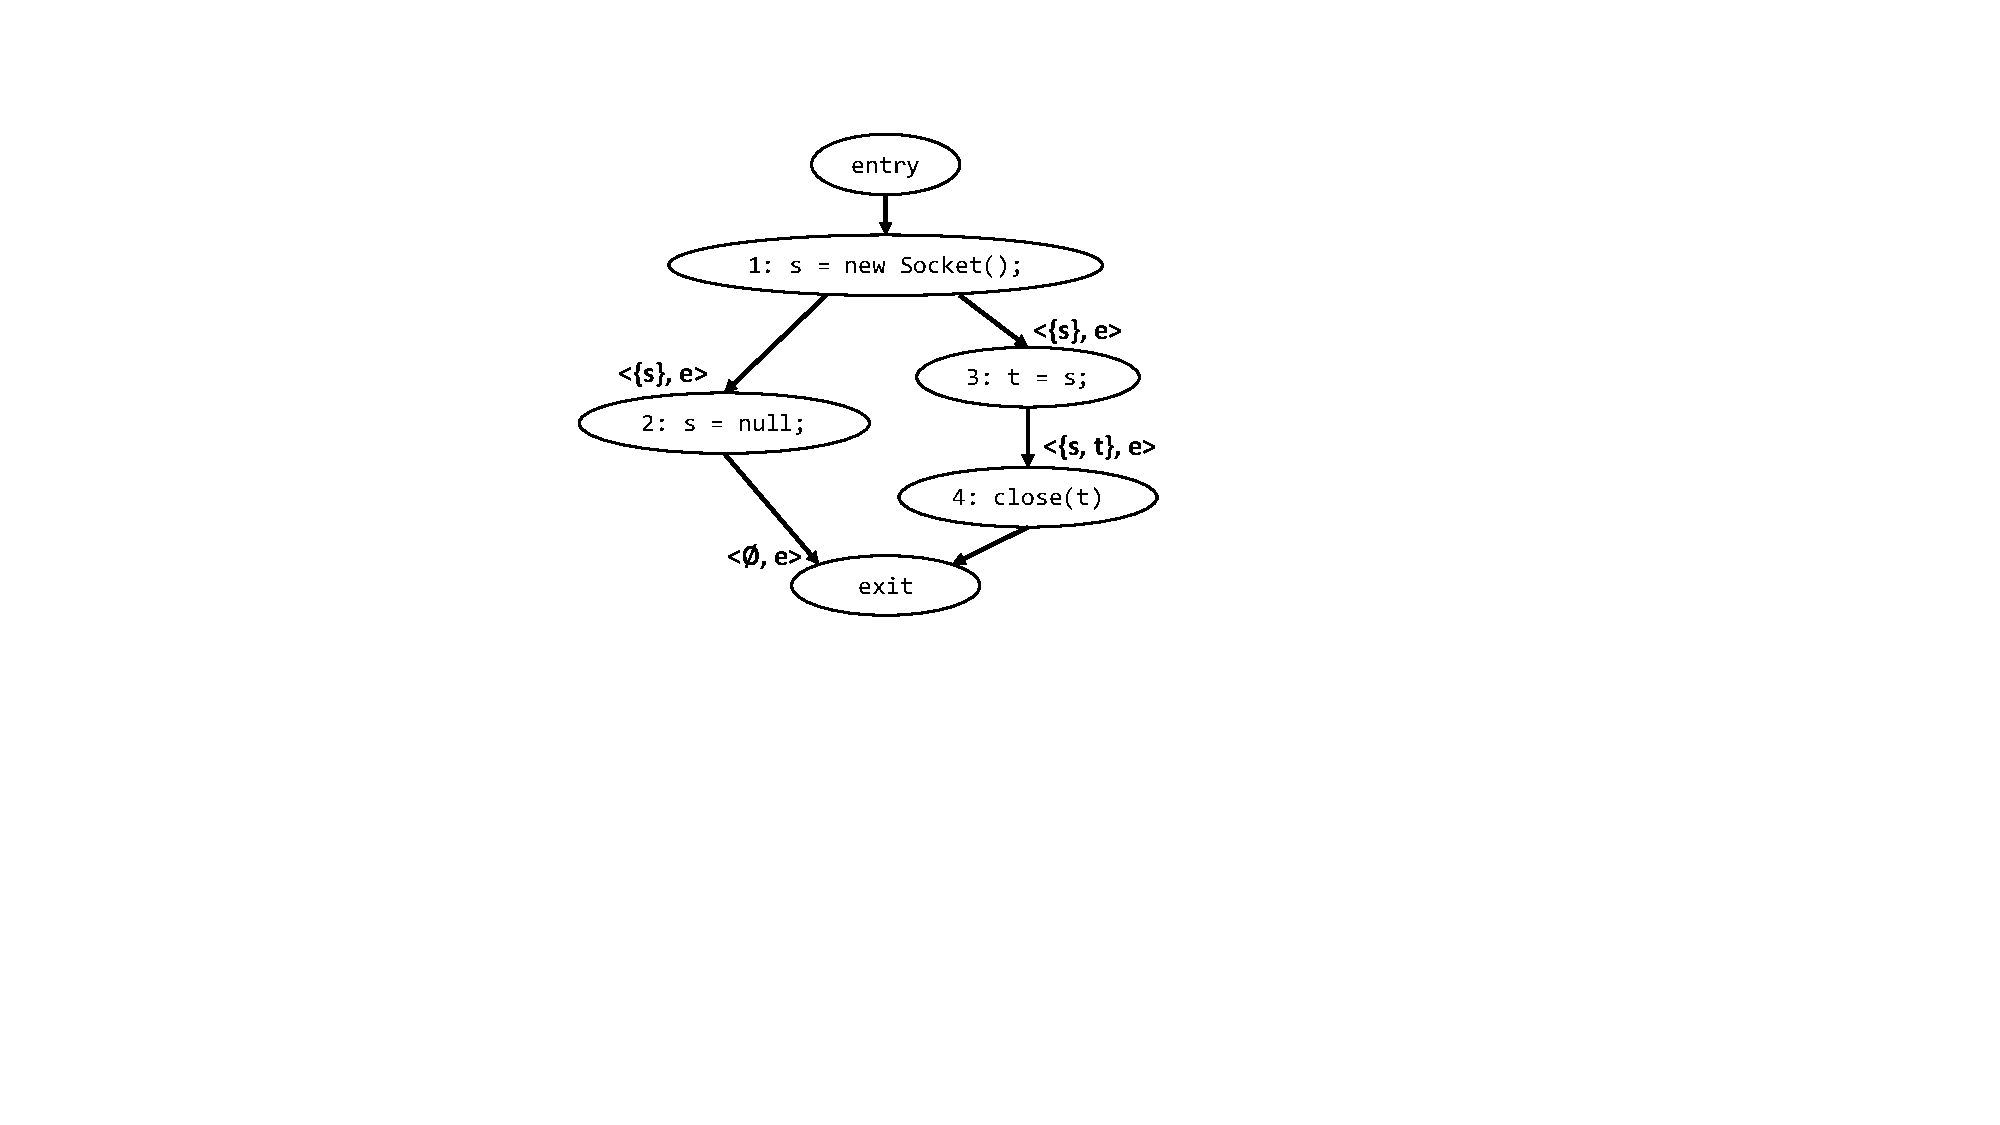
\includegraphics[width=\linewidth,keepaspectratio]{cfg-example.pdf}
  \end{minipage}
  \prefigcaption
  \vspace{-5pt}
  \caption{Example code and CFG for illustrating \cref{alg:consistency-checker}.
    ``\<e>'' is ``\<new Socket(...)>''.
    Non-shaded facts are created by
    %% Commented out to save a line
    % procedure
    \textsc{InitialObligations}, and
    shaded facts are propagated by the fixed-point loop.
} \label{fig:cfg-example}
\end{figure}

\paragraph{Example} To illustrate our analysis, \cref{fig:cfg-example} shows a
simple program (irrelevant details elided) and its corresponding CFG.
The CFG shows the dataflow facts propagated along each edge.
For initialization, statement 1 introduces the fact $\langle \{ s \}, e
\rangle$ (where $e$ is the \<new Socket(...)> call) to $D(2)$ and $D(3)$.  At
statement 2, $s$ is killed, causing $\langle \emptyset , e \rangle$ to be added
to $D(\mathit{exit})$.  This leads to an error being reported for statement 1, as
the socket is not closed on this path.  Statement 3 creates a must alias $t$ for
$s$, causing $\langle \{ s, t \}, e \rangle$ to be added to $D(4)$.  For
statement 4, $\textsc{MCSatisfiedAfter}(\{s,t\},\mathtt{close(t)})$ holds, so no
facts are propagated from 4 to $\mathit{exit}$.

% At this point, we have described a sound checker for \MustCall obligations.
% % But for real code, this checker emits too many false positives.  In particular,
% % the dataflow analysis is purely intra-procedural, and it will report errors in
% % cases where obligations are satisfied via parameter passing, returns, or fields.
% Subsequent sections make the checker more precise.

% The Ownership Checker is a simple worklist algorithm that operates over the CFG.
% It maintains a set of owning pointers to objects, using a set of simple
% ownership rules:
% \begin{itemize}
% \item a newly-allocated object is owned
% \item the value returned by any method called is owned
% \end{itemize}

% These rules guarantee that there is at least one owning pointer to each
% object that might contain a resource. \Cref{sec:lightweight-ownership}
% gives more details on how ownership is transferred.

% When an owning pointer goes out of scope, the Ownership Checker
% compares the types computed by the Must Call Checker and the Called
% Methods Checker to determine if the requirements on the expression
% going out of scope have been fulfilled using the following process,
% supposing that some expression \<expr> is going out of scope at
% program point $P$:
% \begin{enumerate}
%   \item The Ownership Checker requests a Must Call type from the Must
%     Call Checker for \<expr> at $P$. Suppose this type is
%     \MustCall\<(>$A$\<)> for some set of methods $A$ (if the type is
%     \MustCallUnknown, the Ownership Checker always issues an
%     error).
%   \item The Ownership Checker requests a Called Methods type from the
%     Called Methods Checker for \<expr> at $P$. Suppose this type is
%     \<@CalledMethods(>$B$\<)> for some set of methods $B$.
%   \item The Ownership Checker compares the sets $A$ and $B$. If
%     $A \supset B$, the Ownership Checker issues an error.
% \end{enumerate}

% The Ownership Checker also does a simple, intra-procedural must-alias
% analysis, to avoid issuing duplicate errors for e.g. constructor
% invocations that are assigned to local variables. At most one error
% for each must-alias set is ever issued. 

% LocalWords:  simplesocket MustCallUnknown MCAB MustCall MCA xshift MCB
% LocalWords:  yshift Closeable CalledMethods CalledMethodsBottom IsExit
% LocalWords:  FindMissedCalls MCSatisfied CreatesAlias MCObligations p'
% LocalWords:  HasMCReturn EndOfScope CMBefore MCBefore MCAfter
% LocalWords:  CMAfter HasObligation FactsFromCall MCSatisfiedAfter intra
% LocalWords:  InitialObligations worklist xleftmargin makeSocket addr
% LocalWords:  ByteArrayOutputStream


\section{Lightweight ownership tracking}
\label{sec:lightweight-ownership}

\Cref{sec:base-type-systems} describes a sound accumulation-based
checker for resource leaks. However, that checker often encounters false
positives caused by cases where a \<@MustCall> obligation is satisfied
in another procedure, via parameter passing, return values, or object fields.
For example, consider the following code that safely closes a \<Socket>:

\begin{lstlisting}[frame=tb,belowskip=3mm]
  void example(String myHost, int myPort) {
    Socket s = new Socket(myHost, myPort);
    closeSocket(s);
  }
  void closeSocket(@Owning Socket s) {
    s.close();
  }  
\end{lstlisting}

The \<closeSocket()> routine takes ownership of the socket---that is,
it takes responsibility for closing it. The correct place for our
checker to enforce that \<close()> has been called on \<s> is not
when \<s> goes out of scope in \<example()>, but rather when \<s>
goes out of scope in \<closeSocket()>. The checker described by
\cref{sec:base-type-systems} would issue a false positive on this
code, because it would warn about \<example>'s pointer to \<s>.
With the \<@Owning> annotation on the parameter to \<closeSocket>,
however, the checker can determine that \<closeSocket> is the correct
place to check.

Here, we describe a \emph{lightweight ownership tracking} technique for reducing
false positives in such cases.  With lightweight ownership, programmer
annotations \emph{cannot} introduce any checker unsoundness; they can only to
reduce false positives.  Further, unlike other ownership type systems~\todo{cite},
lightweight ownership imposes no restriction on what operations can be performed
through an alias, and hence has a minimal impact on the programming model.

\subsection{Ownership transfer}
\label{sec:ownership-transfer}

With lightweight ownership, a parameter, return, or field type may be annotated
as either \<@Owning> or \<@NotOwning>.  In the Must Call Consistency Checker
(\Cref{sec:must-call-invoked}), if a tracked variable $p$ is assigned to such an
\<@Owning> location $l$, we \emph{transfer} ownership to $l$, and $p$'s
\<@MustCall> obligation is treated as satisfied. Assume we have a helper
function $\textsc{OwningReturn}(CFG)$ that checks if the return type of $CFG$'s
method is \<@Owning>, and $\textsc{PassedAsOwningParam}(s,p)$ that checks if $s$ is a
call that passes $p$ to an \<@Owning> parameter of the callee.  Then,
\textsc{MCSatisfied}$(P,s)$ of \Cref{alg:helpers} is enhanced to handle
ownership transfer as follows:

% \begin{align*}
%   \exists p \in P &.\ \textsc{MCBefore}(p,s) \subseteq \textsc{CMBefore(p,s)}\\
%                   &\vee (s \mathrm{\ is\ } \mathtt{return\ p} \wedge \mathrm{method\ return\ type\ is\ } \mathtt{@Owning})\\
%                   &\vee (s \mathrm{\ is\ } \mathtt{q\ =\ foo(...,p,...)} \wedge \mathtt{p} \mathrm{\ is\ } \mathtt{@Owning})\\
%                   &\vee (s \mathrm{\ is\ } \mathtt{q.f\ =\ p} \wedge \mathtt{f} \mathrm{\ is\ } \mathtt{@Owning})\\
% \end{align*}
\begin{algorithmic}
  \Procedure{MCSatisfied}{$P,s$}
  \State \Return $\exists p \in P .\ \textsc{MCAfter}(p,s) \subseteq \textsc{CMAfter}(p,s)$ \newline
  \hspace*{6em} $\vee\ (s \mathrm{\ is\ } \mathtt{return\ p} \wedge \textsc{OwningReturn}(CFG))$ \newline
  \hspace*{6em} $\vee\ \textsc{PassedAsOwningParam}(s,p)$\newline
  \hspace*{6em} $\vee\ (s \mathrm{\ is\ } \mathtt{q.f\ =\ p} \wedge \mathtt{f} \mathrm{\ is\ } \mathtt{@Owning})$
  \EndProcedure

\end{algorithmic}

To ensure soundness, the analysis must ensure that the \<@MustCall> obligation
of any \<@Owning> location is satisfied.  We discuss checking of \<@Owning>
fields in \Cref{sec:owning-fields}.  For \<@Owning> method returns, we need only
update the \textsc{Has\-MCReturn} routine used in \Cref{alg:helpers} to check that
the return type both has a non-empty \<@MustCall> obligation \emph{and} is
\<@Owning>.  For \<@Owning> parameters, the loop at
Lines~\ref{li:start-init}--\ref{li:end-init} in \Cref{alg:consistency-checker}
must be extended to also add each \<@Owning> formal parameter as a dataflow
fact at the entry node of the CFG.  These relatively simple changes are all that
is required to add lightweight ownership tracking to our technique.\todo{but we
didn't discuss fields yet...}

By default, our checker assumes that unannotated return types are \<@Owning>,
but that parameter and field types are \<@NotOwning>.  These assumptions
coincide well with coding patterns we observed in practice, reducing the
annotation burden for programmers.  Further, this treatment of parameter and
return types ensures sound handling of unannotated third-party libraries: any
object returned from such a library will be tracked by default, and the checker
never assumes that passing an object to a library will satisfy its obligation.

Programmers can override defaults by writing explicit \<@Owning> or
\<@NotOwning> annotations on method returns (constructors are always
\<@Owning>), parameters, and fields (though never both at the same
location---they are mutually exclusive).  Such explicit annotations can
\emph{never} compromise soundness.  If such an annotation is incorrect (e.g., an
\<@Owning> annotation on a reference that does not satisfy an obligation), it
can only lead to false positives, not false negatives.  Due to this design,
there is great scope for creating inference techniques for lightweight
ownership, to further reduce annotation burden; we plan to pursue such
techniques in future work.
\todo{pointer to further discussion in evaluation?}

\todo{Add a para comparing to Rust ownership and the like?}

\subsection{Final owning fields}
\label{sec:owning-fields}

  Additional class-level checking is required for \<@Owning> fields, as the code
  satisfying their \<@MustCall> obligations nearly always spans multiple
  procedures.  We first discuss the case of final fields,\footnote{We only
  consider instance fields in this paper; we have not observed resource leaks
  through static fields in our benchmarks, and we leave their handling to future
  work.} which cannot be overwritten after initialization of the enclosing
  object.  Consider a final \<@Owning> field $f$ declared in class $C$, where
  $f$ has type \<@MustCall("m")>.  To
  verify that $f$'s \<@MustCall> obligation is satisfied, we check the following
  conditions:
  \begin{enumerate}
    \item All $C$ objects must have a type \<@MustCall("n")> for some method $C.n$.
    \item $C.n$ must always invoke \<this.f.m()>, thereby satisfying $f$'s
    \<@MustCall> obligation.
  \end{enumerate}
  In this manner, we verify the usage of $f$, by imposing
  a \<@MustCall> obligation on clients using the $C$ class.  Condition 2 is
  checked by requiring an appropriate \<@EnsuresCalledMethods> annotation on
  $C.n$, which is then enforced by the Called Methods
  Checker~\cite{KelloggRSSE2020}.  \todo{this all needs an example...} \todo{Mention RAII}

  While this scheme suffices for verifying final fields, we observed many cases
  in our benchmarks of non-final fields with \<@MustCall> obligations.  Checking
  non-final fields requires additional techniques, as the checker must ensure
  that overwriting the field does not lead to a \<@MustCall> violation.  We
  describe our novel handling of non-final fields in \Cref{sec:reset-must-call}.


% LocalWords:  MustCall belowskip myHost myPort closeSocket NotOwning
% LocalWords:  MCSatisfied MCBefore CMBefore MCReturn EnsuresCalledMethods


\section{Resource aliasing}
\label{sec:must-call-choice}

This section introduces a lightweight, specialized must-alias analysis
that tracks \emph{resource alias} sets---sets of pointers that
definitely correspond to the same underlying system resource.  Because
resource aliases correspond to the same underlying resource, closing
one alias also closes the other---so our sound resource alias analysis
permits \Tool to avoid issuing false positive warnings about resources
that have already been closed through their resource aliases.  Prior
work on accumulation analyses showed that limited, specialized forms
of alias analysis can provide precision to an accumulation analysis
where needed, without incurring the cost of a whole-program
analysis~\cite{KelloggRSSE2020}; our resource alias analysis is no
different.

\subsection{Wrapper types}

Precise leak detection for Java requires reasoning about \emph{wrapper types},
which wrap another type that may contain a resource.  For example, the Java
\<BufferedOutputStream> type adds buffering to some other \<OutputStream>, which
may or may not represent a resource that needs closing.  Wrapper types
introduce two additional complexities for \<@MustCall> checking:
\begin{enumerate}
  \item If a wrapped object has no \<@MustCall> obligation, the corresponding
  wrapper object should also have no obligation.
  \item Satisfying the obligation of \emph{either} the wrapped object or the
  wrapper object is sufficient.
\end{enumerate}
For example, if a \<BufferedOutputStream> $b$ wraps a stream with no underlying
resource (e.g., a \<ByteArrayOutputStream>), $b$ should have an empty
\<@MustCall> obligation, since $b$ has no resource of its own.  On the other
hand, if $b$ wraps a stream managing a resource, like a \<FileOutputStream> $f$,
then \<close()> must be invoked on \emph{either} $b$ or $f$. Calling \<close()> on $b$
is sufficient since $b$\<.close()> invokes \<close()> on its wrapped stream $f$.

Previous work has shown that a reasoning about wrapper types is
required to avoid excessive false positive and duplicate
reports~\cite{TorlakC10,ecj-resource-leak}.  Wrapper types in earlier
work were handled with hard-coded specifications of which library
types are wrappers and also, in the work of Torlak and
Chandra~\cite{TorlakC10}, a clustering technique to group warnings
involving a resource and its wrappers.

Our technique handles wrapper types more generally by tracking \emph{resource
aliases} during analysis.  Two references $r_1$ and $r_2$ are resource aliases
iff:
\begin{itemize}
\item satisfying $r_1$'s \<@MustCall> obligation also satisfies $r_2$'s
  obligation, and vice-versa; or
\item if $r_1$ and $r_2$ are must-aliased pointers.
\end{itemize}
We also introduce a new type
qualifier \mccannot to indicate where an API method creates a resource-alias
relationship between distinct objects, like a wrapper and the wrapped resource.
\mccannot can be used to annotate a \<BufferedOutputStream> constructor as follows:
\begin{lstlisting}
@MustCallAlias BufferedOutputStream(@MustCallAlias OutputStream arg0);
\end{lstlisting}

\mccannot qualifiers must always appear in pairs---one on a parameter
of a method, and another on its return type.  A pair of \mccannot
annotations has two effects on our inference and checking.  First,
must-call obligation inference (\Cref{sec:must-call}) treats the
annotated elements as polymorphic---the must-call obligations of the
parameter are copied to the return type. Therefore, if the wrapped
type has no must-call obligations (like a \<ByteArrayOutputStream>),
the wrapper will not have must-call obligations, either.

Second, at call sites, the Must Call Consistency Checker
(\Cref{sec:must-call-choice}) treats the \mccannot parameter and return as
aliases.  Specifically, the \textsc{CreatesAlias} routine in \cref{alg:helpers} is
modified as follows \todo{better notation!}:
\begin{algorithmic}
  \Procedure{CreatesAlias}{$P,s$}
    \State \Return $s$ is \lstinline{p = q} $\wedge\ q \in P$ \newline
         \hspace*{4.5em} $\vee$ $(s$ is \lstinline{p = foo(p1, p2, ...)} \newline
         \hspace*{6em} $\wedge\ \exists p_i \in P.\ q_i$ is
         \lstinline{@MustCallAlias} in \lstinline{foo})
    \EndProcedure
\end{algorithmic}
Beyond must-aliasing between local variables, the routine now treats the
assigned variable $p$ of a call statement as a new resource alias if a tracked
variable in $P$ is passed to some \mccannot parameter.
With this change, \Cref{alg:consistency-checker} will treat the case of a
resource alias exactly the same as a standard must alias.
% As shown in
% \cref{alg:consistency-checker}, the returned set is added to the set of tracked
% variables for a resource (\cref{li:compute-new-mc-aliases}), and the algorithm
% treats satisfaction of the \<@MustCall> obligation for any variable in the set
% as satisfying all the others.\todo{need another pass on this prose...}

\subsection{Beyond wrapper types}

\mccannot can also be employed in scenarios beyond direct wrapper types, a
capability not present in previous work.  In certain cases, a resource gets
shared between objects via an intermediate object that cannot directly close the
resource.  For example, \<java.io.RandomAccessFile> (which must be closed) has
a method \<getFd()> that returns a \<FileDescriptor>
object for the file. This file
descriptor cannot be closed directly---it has no \<close()> method.
However, the descriptor can be passed to a wrapper stream such as
\<FileOutputStream>, which if closed satisfies the original must-call
obligation.  By adding \mccannot annotations to the \<getFd()> method, our
technique can verify code like the below (adapted from Apache Hadoop~\cite{hadoop-random-access-file}):
\begin{lstlisting}[frame=tb,belowskip=3mm]
  RandomAccessFile file = new RandomAccessFile(myFile, "rws");
  FileInputStream in = null;
  try {
    in = new FileInputStream(file.getFD());
    // do something with in  
    in.close();
  } catch (IOException e){
    file.close();
  }
\end{lstlisting}
We assign \<FileDescriptor> a special \<@MustCall(?)> type that cannot be satisfied by any calls,
but which is converted back into \<@MustCall("close")> when passed to the \<@MustCallAlias> constructor
of \<FileInputStream>. We found this capability to be
useful for verifying multiple code patterns in our case studies.

\subsection{Verification of \mccannot}

A pair of \mccannot annotations on a method or constructor \<m>'s return type
and its parameter \<p> can be verified via one of two
procedures:
\begin{enumerate}
\item if \<p> is passed to another method or constructor in an
  \mccannot position, and \<m> returns the result of that method
  (or the method is a \<super()> constructor call appropriately annotated
  with \mccannot), then the code can be verified.
\item if \<p> is stored in an \<@Owning> field of the class, and the
  class declaration has an \<@MustCall(>$A$\<)> annotation for some set
  of methods $A$, and at least one of the methods in $A$ has an
  \<@EnsuresCalledMethods> annotation naming at least the
  must-call obligations of \<p>'s static type, then the code can be verified.
\end{enumerate}
These verification procedures permit a programmer to soundly specify a resource-aliasing
relationship in their own code, a capability that was not present in prior work
that relies on a hard-coded list of wrapper types, and that we used in our case studies
\todo{3 in Zookeeper + however many in the rest} times.

% As noted in previous work, p
% The
% must-call obligation for an arbitrary \<BufferedOutputStream> is
% \<@MustCall(\{``close''\})>---the stream might be writing to a file,
% for example.  \<BufferedOutputStream>'s constructors all have a
% parameter which is another \<OutputStream>. When \<close()> is called
% on the resulting \<BufferedOutputStream>, the implementation calls
% \<close()> on the wrapped \<OutputStream>. Since there are no
% additional resources allocated by the \<BufferedOutputStream> that
% were not part of the \<OutputStream> passed to the constructor,
% calling \<close()> on either stream is equally correct (though most
% Java style guides suggest calling \<close()> on the outermost
% wrapper \todo{cite that claim?}).

% Code that uses these streams usually calls \<close()> on only one
% of the streams---either the wrapper stream or the wrapped stream.
% A tool that reported an error for one stream if the other was closed
% would report too many false positives to be usable in practice.
% Prior work uses a pre-determined list of wrapper classes, built into
% the tool, to handle this issue~\cite{TorlakC10}. \todo{Also cite ecj here?
%   I think it also uses the same scheme...}

% LocalWords:  BufferedOutputStream OutputStream MustCall FileOutputStream
% LocalWords:  ByteArrayOutputStream MustCallAlias arg0 CreatesAlias getFd
% LocalWords:  FileDescriptor belowskip RandomAccessFile myFile rws getFD
% LocalWords:  FileInputStream EnsuresCalledMethods


\section{Creating new obligations}
\label{sec:reset-must-call}

%%%%%%%%%%%%%%%%%%%%%%%%%%%%%%%%%%%%%%%%%%%%%%%%%%%%%%%
%% This table is here instead of the evaluation section
%% so that it is placed on the appropriate page.
%%%%%%%%%%%%%%%%%%%%%%%%%%%%%%%%%%%%%%%%%%%%%%%%%%%%%%%

% a line in tab:case-studies
% arguments: project name, original LoC, # of resources (-AcountMustCall), diff size, # of annotations, TPs, Confirmed TPs, FPs, run time in seconds
\newcommand{\osstablerow}[8]{\textbf{\smaller{#1}} & #2 & #3 & #4 & #5 & #6 & #7 & #8}

\begin{table*}
  \caption{
    \todo{Recompute all numbers in the docker image, except wall-clock time.}
    Verifying the absence of resource leaks in case studies.
    % LoC is computed using scc. Be careful when computing LoC to run scc from relevant top-level
    % directory that only contains source code (not test code!) to make sure that the count is accurate.
    % for Zookeeper, this directory is zookeeper/zookeeper-server/src/main/java
    Throughout, ``LoC'' is lines of non-comment, non-blank Java code.
    ``Resources'' is the number of resources created by the program.
    % to compute the diff size, do something like the following (this is what I did for Zookeeper) from the with-annotations branch:
    % > git diff origin/with-checker -- '*.java'
    % then count the number of individual changesets and report that
    ``Annos.'' is number of manually-written annotations to specify
    existing methods.
    ``Code changes'' is the number of distinct changes to program text we made,
    not including changes that will be erased at compile time
    (such as annotations or warning suppressions).
    ``TPs'' is true positives.
    ``FPs'' is false positives, where the our analysis could not
  guarantee that the call was safe, but manual analysis revealed that no
  run-time failure was possible.
  % ``RT(s)'' is the wall-clock run time of our analysis.
  }
  \label{tab:case-studies}
  \posttablecaption

  \begin{tabular}{@{}lrr|rr|rr|r@{}}
    Project:module                                               &      LoC      & Resources   &  Annos.  &  Code changes   & TPs      & FPs & Wall-clock time      \\
    \hline
    \osstablerow{apache/zookeeper:zookeeper-server}                   {45,248}        {171}       {122}          {5}          {13}       {48}   {1m 24s}        \\
    \osstablerow{apache/hadoop:hadoop-hdfs-project/hadoop-hdfs}       {151,595}        {365}       {117}          {9}        {22}        {48}   {16m 21s}        \\
    \osstablerow{apache/hbase:hbase-server, hbase-client}             {220,828}        {55}          {45}          {5}        {5}        {20}   {7m 45s}        \\
    \osstablerow{plume-lib/plume-util}                                {10,393}        {109}          {2}          {19}        {8}        {2}   {0m 15s}        \\
    \hline
    \osstablerow{\textbf{Total}}                                      {428,064}        {700}         {286}          {38}        {48}       {118}   {-}        \\
  \end{tabular}
\end{table*}

Every constructor of a class that has must-call obligations
implicitly creates obligations for the newly-created object.
However, non-constructor methods may also create obligations
when re-assigning non-final, owning fields or allocating
new system-level resources.
A post-condition annotation,
\CreatesObligation,
indicates for which expression an obligation is created.

At each call to a method annotated as \CreatesObligation\<(>\|expr|\<)>, \tool removes any
inferred Called Methods information about \|expr|, reverting to
the declared type of \|expr|.
% if the target's default must-call type includes any
% methods that are not in its the current must-call type, they are added.
Since a \CreatesObligation annotation can only increase its target's obligations,
no verification for them is needed: placing them anywhere in the program is sound
(but may reduce precision).

When checking a call to a method annotated as
\CreatesObligation\<(>\|expr|\<)>, the Must Call Consistency Checker
(1) treats the \MustCall
obligation of \|expr| as \emph{satisfied},
and (2) creates a fresh obligation to check.
%
In terms of our \cref{sec:must-call-invoked} pseudocode,
we can update the \textsc{FactsFromCall} and \textsc{MCSatisfiedAfter} procedures of
\cref{alg:helpers} to handle \CreatesObligation as follows ($[\ldots]$ stands for the cases shown previously,
including those in \cref{sec:ownership-transfer}):
%\todo{I suggest putting the base code first and the addition with COTargets second.}
\begin{algorithmic}
  \Procedure{FactsFromCall}{$s$}
  \State $p \gets s.LHS, c \gets s.RHS$
  \State \Return $\{ \langle \{ p_i \}, c \rangle\ |\ p_i \in \textsc{COTargets}(c) \}$ \newline
  \hspace*{5em} $\cup\ (\textsc{HasObligation}(c)$ ? $\{ \langle \{ p \}, c \rangle \}$ : $\emptyset)$
  \EndProcedure
  \Procedure{MCSatisfiedAfter}{$P,s$}
  \State \Return $\exists p \in P .\ [\ldots] \vee p \in \textsc{COTargets}(s)$
  \EndProcedure
  \Procedure{COTargets}{$c$}
  \State \Return \{ $p_i$\ |\ $p_i$ passed to a \CreatesObligation target for $c$'s callee \}
  \EndProcedure
\end{algorithmic}
\noindent
This change is sound: the checker creates a new obligation for calls to
\CreatesObligation methods, and the must-call obligation checker (\cref{sec:must-call}) ensures the
\MustCall type for the target will have a \emph{superset} of any methods present
before the call.
There is an exception to this check: if an \CreatesObligation
method is invoked within a method that has an \CreatesObligation annotation
with the same target---imposing the obligation on its caller---then
the new obligation can be treated as satisfied immediately.\looseness=-1

\subsection{Non-final, owning fields}
\label{sec:non-final-owning}

\CreatesObligation allows \tool to verify uses of non-final fields
that contain a resource, even if they are re-assigned. Consider
the following example:

\begin{lstlisting}[frame=tb,belowskip=3mm]
  @MustCall("close") // default qualifier for uses of SocketContainer
  class SocketContainer {
    private @Owning Socket sock;
    public SocketContainer() { sock = ...; } 
    void close() { sock.close() };
    @CreatesObligation("this")
    void reconnect() {
      if (!sock.isClosed()) {
        sock.close();
      }
      sock = ...;
    }
  }
\end{lstlisting}
In the lifetime of a \<SocketContainer> object, \<sock>
might be re-assigned arbitrarily many times: once at each
call to \<reconnect()>. This code is safe, however: \<reconnect()>
ensures that \<sock> is closed before re-assigning it.

\Tool must enforce two new rules to ensure that
re-assignments to non-final, owning fields like \<sock> in the example
above are sound:
\begin{itemize}
\item any method that re-assigns a non-final, owning field of an object
  must be annotated with an \CreatesObligation annotation
  that targets that object.
\item when a non-final, owning field $f$ is re-assigned at statement $s$,
  its inferred \MustCall obligation must be contained in its \<@CalledMethods>
  type at the program point before $s$.
\end{itemize}
\noindent
The first rule ensures that \<close()> is called after the last call
to \<reconnect()>, and the second rule ensures that \<reconnect()>
safely closes \<sock> before re-assigning it. Because calling
an \CreatesObligation method like \<reconnect()> resets called-methods
inference, calls to \<close> before the last call to \<reconnect()>
are disregarded.

\subsection{Unconnected sockets}
\label{sec:unconnected-sockets}
\CreatesObligation can also handle cases where object creation
does not allocate a resource, but the object will allocate a resource
later in its lifecycle. Consider the no-argument constructor
to \<java.net.Socket>. This constructor does not allocate an
operating system-level socket, but instead just creates the container
object, which permits the programmer to e.g. set options which will be used
when creating the physical socket. When such a \<Socket> is created, it
initially has no must-call obligation; it is only when the \<Socket> is
actually connected via a call to a method such as \<bind()>
or \<connect()> that the must-call obligation is created.

If all \<Socket>s are treated as \MustCall\<(\{"close"\})>,
a false positive would be reported
in code such as the below, which operates on an unconnected socket
(simplified from real code in Apache Zookeeper~\cite{zookeeper-create-socket}):

\begin{lstlisting}[frame=tb,belowskip=3mm]
  static Socket createSocket() {
    Socket sock = new Socket();
    sock.setSoTimeout(...);
    return sock;
  }
\end{lstlisting}

\noindent
The call to \<setSoTimeout> can throw a \<SocketException> if the
socket is actually connected when it is called. Using \CreatesObligation,
however, \tool can soundly show that this socket is not connected:
the type of the result of the no-argument constructor can be
treated as \<@MustCall(\{\})>, and \CreatesObligation annotations
on the methods that actually allocate the socket---\<connect()> or
\<bind()>---enforce that as soon as the socket is actually open,
it is treated as \<@MustCall("close")>.

% LocalWords:  belowskip MustCall SocketContainer sc CreateObligation expr
% LocalWords:  RMCTargets MCObligations HasMCReturn MCSatisfied COTargets
% LocalWords:  createSocket setSoTimeout SocketException FactsFromCall
% LocalWords:  MCSatisfiedAfter CreateObligation isClosed CalledMethods


\section{Implementation}
\label{sec:implementation}

\todo{Any paper that involves building a tool should include an ``implementation'' section.
  It may discuss a new tool you have built and/or the experimental infrastructure.
  Discuss the key non-obvious design decisions and complications.
  You should also mention: 1) what language the tool targets, 2) any important libraries that
  the tool relies on (\eg the Checker Framework), and 3) that the tool is
  open-source.

  Sometimes this section is very short.}


\section{Evaluation}
\label{sec:evaluation}

% TODO: if this table is after tab:case-studies, then it doesn't appear? WTF


% a line in tab:case-studies
% arguments: project name, original LoC, # of resources (-AcountMustCall), diff size, # of annotations, TPs, Confirmed TPs, FPs, run time in seconds
\newcommand{\osstablerow}[8]{\textbf{\smaller{#1}} & #2 & #3 & #4 & #5 & #6 & #7 & #8}

\begin{table*}
  \caption{Verifying the absence of resource leaks in case studies.
    % LoC is computed using scc. Be careful when computing LoC to run scc from relevant top-level
    % directory that only contains source code (not test code!) to make sure that the count is accurate.
    % for Zookeeper, this directory is zookeeper/zookeeper-server/src/main/java
    Throughout, ``LoC'' is lines of non-comment, non-blank Java code.
    ``Resources'' is the number of resources created by the program.
    % to compute the diff size, do something like the following (this is what I did for Zookeeper) from the with-annotations branch:
    % > git diff origin/with-checker -- '*.java'
    % then count the number of individual changesets and report that
    ``Annos.'' is number of manually-written annotations to specify
    existing methods.
    ``Code changes'' is the number of distinct changes program text we made,
    not including changes that will be erased at compile time
    (such as annotations or warning suppressions).
    ``TPs'' is true positives.
    ``FPs'' is false positives, where the our analysis could not
  guarantee that the call was safe, but manual analysis revealed that no
  run-time failure was possible.
  % ``RT(s)'' is the wall-clock run time of our analysis.
  }
  \label{tab:case-studies}
  \posttablecaption

  \begin{tabular}{@{}lrr|rr|rr|r@{}}
    Project:module                                               &      LoC      & Resources   &  Annos.  &  Code changes   & TPs      & FPs & Wall-clock time      \\
    \hline
    \osstablerow{apache/zookeeper:zookeeper-server}                   {45,410}        {232}       {98}          {5}          {12}       {47}   {1m 24s}        \\
    \osstablerow{apache/hadoop:hadoop-hdfs-project/hadoop-hdfs}       {151,233}        {366}       {129}          {7}        {22}        {37}   {16m 21s}        \\
    \osstablerow{apache/hbase:hbase-server, hbase-client}             {170,569}        {62}          {35}          {1}        {11}        {27}   {7m 45s}        \\
    \hline
    \osstablerow{\textbf{Total}}                                      {563,855}        {660}         {262}          {13}        {45}       {111}   {-}        \\
  \end{tabular}
\end{table*}


Our evaluation has three parts:
\begin{itemize}
\item case studies on open-source projects, which show that our approach
  is scalable and finds real bugs (\cref{sec:case-studies}).
\item an evaluation of the contributions of our enhancements:
  lightweight ownership, % (\cref{sec:lightweight-ownership}),
  resource aliasing, % (\cref{sec:must-call-choice}), and
  and obligation creation % (\cref{sec:reset-must-call})
  (\cref{sec:ablation}).
\item a comparison to previous leak detectors:  both heuristic bug-finding
  and heavy-weight whole-program
  % typestate
  analysis (\cref{sec:compare}).
\end{itemize}

\subsection{Case studies on open-source projects}
\label{sec:case-studies}

We selected 3 popular open-source projects that were analyzed by prior work~\cite{zuo2019grapple}.
For each project, we selected and analyzed one or two modules
containing significant uses of leakable resources. We used
the latest version of the source code that was available
when we analyzed the code.

Our methodology was:
(1)
We modified the
build system to run our analysis on the module, analyzing uses of resource
classes that are defined in the JDK\@.
It also reports the maximum possible number of resources that could be
leaked:  each obligation at a formal parameter or method call.
(2) We manually
annotated each program with must-call, called-methods, and ownership
annotations (see \cref{sec:annos}).
The
annotated versions of the case study programs (including
the commit hashes that we analyzed) are available at
\todo{an anonymized fork of the projects}.
% the ``Annos'' column in \cref{tab:case-studies}).
(3) We iteratively ran the analysis to correct our annotations.
We measured the run time
as the median of 5 trials on
% This is Mike's home machine.  Are there any other relevant parameters?
a machine with an Intel Core i7-10700 CPU running at 2.90GHz and 64GiB of RAM\@.
Our analysis is embarassingly parallel, but our implementation is
single-threaded because javac is single-threaded.
(4) We manually categorized each warning as revealing a
real resource leak (a true positive or TP) or as correct code that our
system is unable to prove correct (a false positive or FP\@).

\Cref{tab:case-studies} summarizes the results. \Tool found multiple
serious resource leak bugs in every program. \Tool issues
more false positives than true positives in each program, but
the number is small enough to be examined by a single developer in a
few hours.  This is a small price to pay for knowing that the program is
free of resource leaks.  The annotations in the program are
also a benefit: as a form of machine-checked documentation, they
express the programmer's intent and, unlike traditional comments,
cannot become out-of-date if the checker is passing.

\subsubsection{True and false positive examples}
\label{sec:examples}

This section describes some examples of warnings reported by \Tool
in our case studies.\looseness=-1

\begin{figure}
  \lstinputlisting{hadoop-bug.txt}
  \prefigcaption
  \caption{A true positive that \Tool found in Hadoop. Our pull request
    to fix this bug was accepted by Hadoop's developers.}
  \label{fig:hadoop-bug}
\end{figure}

\Cref{fig:hadoop-bug} contains code from Hadoop. If an IO error
occurs any time between the allocation of the \<FileInputStream>
in the first line of the method and the \<return> statement
at the end---for example, if \<channel.position(section.getOffset())>
throws an \<IOException>, as it is specified to do---then the
only reference to the stream is lost. Hadoop's developers
assigned this bug a priority of ``Major'' and accepted our
patch.\footnoteanonurl{https://github.com/apache/hadoop/pull/2652}
One developer suggested using a try-with-resources statement instead
of our patch (which catches the exception and closes the stream),
but we pointed out that
the file needs to remain open if no error occurs so that it can be
returned.  \manu{this example is also interesting in that verifying the caller
is non-trivial.  dunno if we have space, but if we do, we may want to include}
\todo{say something like we are in the process of submitting more bug reports and fixes?}  

\begin{figure}
  \lstinputlisting{zookeeper-optional.txt}
  \prefigcaption
  \caption{Code from the ZooKeeper case study that causes \Tool
  to issue a false positive.}
  \label{fig:zookeeper-optional}
\end{figure}

The most common false
positive pattern (with 15 instances) was caused by
a generic container object like \<java.util.Optional> taking ownership of a resource, such
as the example in \cref{fig:zookeeper-optional}. Our lightweight ownership
system does not support transferring ownership to generic parameters,
so \Tool issues an error when \<Optional.of> is returned. In this case, the use
of the \<Optional> class complicates the code; if \<Optional> was replaced
by \<null>,
%% Leave out of submitted version.
% as some advocate~\cite{ErnstNothingIsBetterThanOptional},
\Tool could verify this code. We leave expanding the lightweight ownership system to
support Java generics as future work.

Most false positives were caused by unique coding patterns.
One example is a series of catch
statements, each of which set an \<error> boolean to \<true>, followed
by a \<finally> statement that closed the relevant socket if \<error>
was true.  \Tool reports an error because it cannot reason about arbitrarily
complex path conditions.


\subsubsection{Annotations and code changes}
\label{sec:annos}

%% Here's the full table of annotations:

%% -              ZK  HB  HD  Total
%% Owning         28  12  43  83
%% NotOwning      8   5   17  30  = 113
%% ----
%% MustCall       13  7   11  31
%% InheritableMC  1   2   7   9   = 41
%% ---
%% MustCallChoice 4   0   28  34
%% PolyMustCall   4   0   0   4   = 36
%% ---
%% ResetMustCall  19  5   5   29  = 29
%% ---
%% EnsuresCM      21  4   18  43  = 43


\begin{table}
  \caption{The total number of annotations that we wrote.}
  \label{tab:annos}
  \posttablecaption
  % counts @InheritableMustCall as @MustCall, for simplicity of presentation
  % counts @polymustcall with MCC, for the same reason
  \begin{tabularx}{\columnwidth}{@{}Xr@{}}
    Annotation                           &      Count     \\
    \hline
    \<@Owning> and \<@NotOwning>            &      113   \\
    \<@EnsuresCalledMethods>                &      43       \\
    \<@MustCall>                            &      41       \\
    \<@MustCallAlias>                       &      36       \\
    \CreateObligation                       &      29      \\
  \end{tabularx}
\end{table}

% Because most relevant \MustCall and \<@CalledMethods> annotations
% are inferred intra-procedurally, most annotations that we had to write in
% the case studies pertained to ownership or the side-effects of procedures.
We wrote less than one annotation per 2,000 lines of code (\cref{tab:annos}).

\todo{Double-check all numbers.}
We also
made 13 small, semantics-preserving changes to the programs to reduce
false positives from our analysis.
%
In 8 places, we added \<final> to a field; this allows our checker to verify it without using
the rules for non-final owning fields given in \cref{sec:reset-must-call}, which are stricter.
In 3 of those, we also removed assignments to the field after it was closed whose right-hand
side was \<null>; in 1 other we added an \<else> clause in the constructor that assigned the field
a \<null> value.
%
In 3 places, we re-ordered two statements to remove an
infeasible control-flow-graph edge.
% In 2 places, we re-ordered a \<try> statement and a null-check.
% % In 1 place, we re-ordered two calls to \<close()> that closed
% the same resource (via resource aliases). The first call in the
% unmodified code was conditional, but the second was
% not, leading to an infeasible control-flow graph edge.
%
In 2 places, we extracted an expression into a local variable, permitting
flow-sensitive reasoning or targetting by a \CreateObligation annotation.
% multiple calls to a method
% into a single call that is assigned to a local variable; this allows
% flow-sensitive reasoning about the local
% variable.
% % , and the code is also more efficient.
% In 1 place, we extracted an expression into a local variable
% so that a \CreateObligation annotation could target it.


\subsection{Evaluating our enhancements}
\label{sec:ablation}

% a line in tab:ablation
% note that the FULL column is always zero, so it's not included here
% arguments: project name, no-LO, no-RA, no-AF
\newcommand{\abltablerow}[4]{\textbf{\smaller{#1}} & #2 & #3 & #4}

\begin{table}
  \caption{The contribution of the lightweight
    ownership, resource aliasing,
    and our system for creating obligations at points other than constructors
    in reducing false positives. Each entry is the number of extra
    false positive warnings reported by the variant with the given feature disabled on the given project.}
  \label{tab:ablation}
  \posttablecaption
  
  \begin{tabularx}{\columnwidth}{@{}Xrrr@{}}
    Project                              &      without LO & without RA & without CO     \\
    \hline
    \abltablerow{apache/zookeeper}              {66}            {97}             {10}                               \\
    \abltablerow{apache/hadoop}                   {95}            {113}             {0}                               \\
    \abltablerow{apache/hbase}                  {52}            {57}             {0}                               \\
    \hline
    \abltablerow{\textbf{Total}}                {213}            {267}             {10}                               \\
  \end{tabularx}
\end{table}

The base analysis of \cref{sec:base-type-systems} produces significantly
more false positives, because it lacks 
lightweight ownership (\cref{sec:lightweight-ownership}),
resource aliasing (\cref{sec:must-call-choice}), and
creating obligations at points other than constructors (\cref{sec:reset-must-call}).
Each contributes to \Tool's precision by eliminating false positives.
To evaluate the contribution of each enhancement, we individually disabled each
feature and re-ran the experiments of \cref{sec:case-studies}.
Since all variants are sound (no false
negatives), any difference in warnings is a false positive that is prevented
by the feature.

\Cref{tab:ablation} shows that each of lightweight
ownership and resource aliases prevents more false positive errors than the total number
of remaining false positives on each benchmarks---showing that removing either
would make our technique produce an unreasonable number of false positives.
The system for creating new obligations at points other than constructors reduces
false positives by a smaller amount: non-final, owning field re-assignments are rare;
and we encountered the unconnected socket pattern described in \cref{sec:unconnected-sockets}
only in ZooKeeper. Nevertheless, this feature allows our tool to handle an important, if rare,
coding pattern.

\subsection{Comparison to other tools}
\label{sec:compare}

Our approach represents a novel point in the design space of resource leak checkers.
%
This section compares our approach with two other modern tools that detect resource leaks:
\begin{itemize}
\item The analysis built into the Eclipse Compiler for Java (ecj), which is the default approach
  for detecting resource leaks in the Eclipse IDE~\cite{ecj-resource-leak}.
\item Grapple~\cite{zuo2019grapple} represents a significant, recent
  improvement in the scalability of typestate-based tools that require a whole-program alias analysis.
\end{itemize}
In brief, both tools are unsound.
Both tools are applicable to legacy code. % , without the need to write annotations.
Eclipse is very fast (nearly instantaneous) and suffers 67--98\% false
positives. % while missing 70-90\% of resource leaks.
According to its authors, Grapple is precise (13\% false positive rate) but orders
of magnitude slower than \Tool.
Different users can select whichever tool matches
their priorities.


\subsubsection{Eclipse}
\label{sec:eclipse}

The Eclipse analysis is a simple dataflow analysis
augmented with heuristics. Because it is tightly integrated with
the compiler, it scales well and runs quickly. It contains
heuristics for ownership, resource wrappers, and resource-free
closeables, among others; these are all hard-coded into the analysis and cannot
be adjusted by the user. It does not support annotations to express
specifications that differ from its defaults.
It supports two levels of analysis: detecting high-confidence resource
leaks and detecting ``potential'' resource
leaks (a superset of high-confidence resource leaks).

We ran this analysis on the same version of Zookeeper's zookeeper-server
module that we ran \Tool on in \cref{sec:case-studies}. It is easy to apply
to legacy code and it is fast---nearly instantaneous once Eclipse
has loaded the project.

In ``high-confidence'' mode on zookeeper-server, Eclipse reports 3
warnings: 1 true positive (thus, it misses 9 real resource leaks) and 2
false positives.
In ``potential'' leak mode, the analysis reported 180
warnings:  3 true positives (it misses 7 real resource leaks) and 177 false
positives.
The most common cause of false
positives was the unchangeable, default ownership transfer assumption
at method invocations: it warned at each call that returns a resource-alias, such as
\<Socket\#getInputStream>.

These results demonstrate that the Eclipse bug-finder is unsound in both
modes: it misses 7 real warnings. Further, the analysis is imprecise: in potential leak mode,
the vast majority of warnings are false positives. However, this sort
of bug-finding tool does have two advantages: it is fast, and it is easily
applicable to legacy code. Compared to our tool, the Eclipse analysis
is much faster and equally applicable to legacy code, but both less sound
and less precise.

%% Chandra rightly pointed out that this para make us look lazy. Let's just
%% say what we did, not why we did it.
%%
%% Given that these results on zookeeper-server
%% clearly show the strengths and weaknesses of this tool compared to our own,
%% we did not run it on our other case study programs.

\subsubsection{Grapple}
\label{sec:grapple}

% a line in tab:grapple
% these numbers come from tables 2 and 3 in the grapple paper from EuroSys.
% for TPs and FPs, I added together the IO and Socket columns of table 2.
\newcommand{\grappletablerow}[4]{\textbf{\smaller{#1}} & #2 & #3 & #4}

\begin{table}
  \caption{The Grapple tool's performance; reproduced from~\cite{zuo2019grapple}.}
  \label{tab:grapple}
  \posttablecaption
  
  \begin{tabularx}{\columnwidth}{@{}Xrrr@{}}
    Project                              &  TPs    &    FPs         & Run time      \\
    \hline
    \grappletablerow{ZooKeeper}             {6}         {0}           {01h 07m 02s}     \\
    \grappletablerow{HDFS}                  {5}         {2}           {01h 54m 52s}    \\
    \grappletablerow{HBase}                 {15}        {2}           {33h 51m 59s}     \\
    \hline
    \grappletablerow{\textbf{Total}}        {26}        {4}           {-}          \\
  \end{tabularx}
\end{table}

% \todo{Be very sure that Grapple is unsound - read their paper again, and
%    point out why in this paragraph.}
%\todo{be sure to note that Grapple is not modular, unlike us}
Grapple~\cite{zuo2019grapple} is a modern typestate-based resource leak analysis
focused on high precision and (relative) scalability. Grapple models its alias and
dataflow analyses as dynamic transitive-closure computations over graphs, and
leverages novel path encodings and techniques from predecessor-system
Graspan~\cite{wang2017graspan} to achieve both context- and path-sensitivity.  
% Grapple, like all previous
% typestate-based analyses, requires a whole-program alias analysis.
Grapple contains four checkers, of which two are useful for detecting
resource leaks.  Unlike \Tool, Grapple is unsound; e.g., it performs a fixed bounded unrolling
of loops to make path sensitivity tractable.

The Grapple authors have already evaluated their tool on earlier
versions\todo{Why don't we repeat our experiments on those earlier versions?
This should be easy to do since it's only a few hours of work and we are now
familiar with the programs.} of the case study programs in
\cref{sec:case-studies}~\cite{zuo2019grapple}; \Cref{tab:grapple} reproduces the
results from their paper.  Based on these numbers, Grapple reports fewer false
positives than \Tool.  Unfortunately, we were not able to successfully run
Grapple's leak detection, and full details on their true and false-positive
warnings are currently unavailable (we have requested them from the authors), so
we cannot study the precision differences further.  The run times in
\Cref{tab:grapple} show a stark difference with our work; \Tool runs in minutes,
whereas Grapple can take many hours. Further, to our best knowledge, Grapple is
not modular, so any code modification will necessitate a full re-analysis.
\Tool only needs to re-analyze modified code and possibly its dependents after
a change, not unmodified dependencies.

% We requested the analysis and Grapple's output, but as of this writing
% (months later) the Grapple authors have not yet provided them.
% \manu{I think this is strictly-speaking true but a bit harsh.  We
% may want to tone it down a bit.}

\todo{Still keep this?} Note that the TP and FP numbers not perfectly comparable between a modular
and a whole-program analysis.
Our tool reports violations of a user-supplied specification
(which takes effort to write but provides documentation benefits), so it
can ensure that a library is correct for all possible clients.  By
contrast, Grapple checks a library in the context of one specific client.

% LocalWords:  LoC SHAs leakable


\section{Limitations and threats to validity}
\label{sec:threats}

Like any tool that analyzes source code, \tool only
gives guarantees for code that it checks: the guarantee
excludes native code, the implementation of unchecked libraries (such as the JDK),
and code generated dynamically or by other annotation processors
such as Lombok.
%% MK: the sentence says that we can't guarantee that code generated by annotation
%% processors is checked, which is true, because they can misbehave in the way
%% that Lombok does. Most annotation processors don't, but the point is that
%% they can, so we can't promise that our analysis will be applied.
%% \todo{nit: is it annotation processors in general that cause an
%% issue, or Lombok because of the insane things it does?  I think for a typical
%% annotation processor doing code generation we shouldn't have problems?}
Though
the Checker Framework can handle 
reflection soundly~\cite{BarrosJMVDdAE2015}, by default (and in our case studies)
\tool compromises this guarantee
by assuming that objects returned by reflective invocations
do not carry must-call obligations.  (Users can customize this behavior.)
% Like any sound static analysis, \Tool does
% issue some false positives; these must be suppressed by
% the programmer and the correctness of the relevant code
% must be proved using another method.
Within the bounds
of a user-written warning suppression, \tool assumes that 1)
any errors issued can be ignored, and 2) all annotations
written by the programmer are correct.

\Tool is sound with respect to specifications of which types have a
\<@MustCall> obligation that must be satisfied.  We wrote such specifications
for the Java standard library, focusing on IO-related code in the \<java.io> and
\<java.nio> packages.  Any missing specifications of \<@MustCall> obligations
could lead \tool to miss resource leaks.

The results of our experiments may not generalize, compromising the
external validity of the experimental results.
% In particular, our subject programs are
% heavily-used, heavily-tested, and contain a high-density of resource
% usage---so, in a sense, they represent a worst-case scenario for
% \tool.  Nevertheless,
\Tool may produce more false positives, require
more annotations, or be more difficult to use if applied to other
programs.
Case studies on legacy code represents a worst case for a source code
analysis tool.  Using \tool from
the inception of a project would be easier, since programmers know their
intent as they write code and annotations could be written along with the
code.  It would also be more useful, since it would guide the programmers
to a better design that requires fewer annotations and has no resource leaks.
The need for annotations could be viewed as a limitation of our approach.
However, the annotations serve as concise documentation of
properties relevant to resource leaks---and unlike traditional, natural-language
documentation, machine-checked annotations cannot become out-of-date.

Like any practical system, it is possible that there might
be defects in the implementation of \tool or in the design of
its analyses. We have mitigated this threat with code review and an extensive
test suite:
% to collect these numbers, run these commands and sum the results:
% cd object-construction-checker/tests
% scc mustcall socket nolightweightownership mustcall-onlyjdk noresourcealias noaccumulationframes
% cd ../../must-call-checker/tests
% scc
119 test classes containing 3,776 lines of non-comment, non-blank code.
This test suite is publicly available and distributed with \tool.

% LocalWords:  checkable MustCall io nio


\section{Related Work}
\label{sec:relatedwork}

Previous work on resource leak detection has typically been based on either
using program analysis to detect leaks or adding language features to prevent
them. Here we discuss the most relevant work from each of these categories.

\subsection{Analysis-based approaches}\label{sec:rw-analysis}

%\todo{Re-organize and edit the below in a way that makes sense.}

\paragraph{Static analysis}
Tracker~\cite{TorlakC10} performs inter-procedural dataflow analysis to detect
resource leaks, with various additional features to make their tool practical,
including issue prioritization and handling of wrapper types.  Tracker avoids
whole-program alias analysis to improve scalability, instead using a local,
access-path-based approach.  While Tracker scales well to large programs, it is
deliberately unsound, unlike \Tool.

The Eclipse Compiler for Java includes a simple dataflow-based
bug-finder for resource leaks~\cite{ecj-resource-leak}. Their analysis
uses a fixed set of ownership heuristics and a fixed list of wrapper
classes; unlike \Tool, it is unsound. It is fast.  Similar analyses---with similar trade-offs
compared to \Tool---are present in other heuristic bug-finding tools,
including SpotBugs~\cite{spotbugs-resource-leak},
PMD~\cite{pmd-resource-leak}, and Infer~\cite{infer-resource-leak}.
\Cref{sec:eclipse} experimentally evaluates the Eclipse analysis.

Typestate analysis~\cite{StromY86,FinkYDRG2008} can be used to
find resource leaks.  Grapple~\cite{zuo2019grapple} is the most recent system to
use this approach, leveraging a disk-based graph engine to achieve unprecedented
scalability on a single machine.  Compared to \Tool, Grapple is more precise but suffers
from unsoundness and much longer run times.
\Cref{sec:grapple} gives a more detailed comparison to Grapple.

Relda and Relda2~\cite{guo2013characterizing,wu2016relda2} are unsound
resource-leak detection approaches \todo{similar to Eclipse,then?} that are
augmented with call graphs to model the Android framework's use of callbacks for
releasing resources.

The CLOSER~\cite{dillig2008closer} automatically inserts Java code to dispose of
resources when they are no longer ``live'' according to its dataflow analysis.
Their approach requires an expensive alias analysis for soundness, as well as
manually-provided aliasing specifications for linked libraries.
\todo{\Tool requires that too, though only lightweight specifications.
  Mention that?}
\Tool uses accumulation
analysis~\cite{KelloggRSSE2020,FahndrichLeino03} to achieve soundness without
the need
for a whole-program alias analysis.
We
build on the core analysis described in~\cite{KelloggRSSE2020}.

\paragraph{Dynamic analysis}
Some approaches use dynamic analysis to ameliorate leaks.  Resco \cite{dai2013resco}
operates similarly to a garbage collector, tracking resources whose program
elements have become unreachable. When a given resource (such as file
descriptors) is close to exhaustion, the runtime runs Resco to clean up any
resources of that type that are unreachable.  With a static approach such as
ours, a tool like Resco becomes unnecessary---leaks become impossible.

Automated test generation can also be used to try to detect resource
leaks. For example, leaks in Android applications can be found by
repeatedly running neutral---eventually returning to the same
state---GUI actions~\cite{wu2018sentinel,zhang2016automated}.
Other techniques focus on taking advantage of common misuse of
the Android activity lifecycle~\cite{amalfitano2020memories}.
Testing can only show the presence of bugs, not their absence;
\Tool verifies that no resource leaks are present.

\paragraph{Data sets and surveys}
In terms of data sets for leak detection, The DroidLeaks
benchmark~\cite{liu2019droidleaks} is a set of Android apps with known resource
leak bugs. Unfortunately, it includes only the compiled apps.
\Tool runs on source code, so we were unable to run \Tool on DroidLeaks.

\todo{This~\cite{ghanavati2020memory} is a recent study on what kinds
  of resource and memory leak bugs happen in large Java projects. I'm
  sure we can use it somewhere.}



\subsection{Language-based approaches}\label{sec:rw-language}

\paragraph{Ownership types and Rust} Ownership type
systems~\cite{clarke2013ownership} impose control over aliasing, which
in turn enables guaranteeing other high-level properties, like absence of
resource leaks.  We do not discuss the vast literature on ownership type systems
here (see Clarke et al.~\cite{clarke2013ownership} for a survey). Instead, we
focus on ownership types in Rust~\cite{klabnik2018rust} as the most popular
practical example of using ownership to prevent resource leaks.

For a detailed overview of ownership in Rust, see Chapter 4
of~\cite{klabnik2018rust}; we give a brief overview here.  In Rust, ownership is
used to manage both memory and other resources.  Every value associated with a
resource must have a \emph{unique} owning pointer, and when an owning pointer's
lifetime ends, the value is ``dropped,'' ensuring all resources are freed.
Rust's ownership type system statically prevents
not only resource leaks, but also other important issues like ``double-free'' bugs
(releasing a resource more than once) and ``use-after-free'' bugs (using a
resource after it has been released). However, this power comes with a cost; to
enforce uniqueness, non-owning pointers must be invalidated after an ownership transfer,
and can no longer be used to perform any operations.  Maintaining multiple
usable pointers to a value requires use of language features like references and
borrowing, and even then, borrowed pointers have restricted privileges.

\Tool has less power than Rust's ownership types; it cannot prevent resources
from being closed multiple times or being used after they are closed.  However,
\Tool's lightweight ownership annotations impose \emph{no} restrictions on
aliasing; they are simply an aid to help the tool identify how a resource will
be closed.  Hence, lightweight ownership is much better suited to preventing
resource leaks in existing, large Java code bases; adapting such programs to use
a full Rust-style ownership type system would be an enormous and impractical
undertaking.

\paragraph{Other approaches} Compensation stacks~\cite{WeimerN04}
generalize C++ destructors and Java's
try-with-resources, to avoid resource leak problems in Java.  While
compensation stacks make resource leaks less likely, they do not provide a
guarantee that leaks will not occur, unlike \Tool.

An alternative to applying a typestate analysis to an existing program
is to rewrite the program in a typestate-oriented programming
language~\cite{AldrichSSS2009,garcia2014typestate}.  The type systems of such
languages are expressive enough to prevent resource leaks, but they impose
restrictions on aliasing and a high type annotation burden, making translation
of existing code impractical.

%\todo{Is there other relevant related work? Find out.}

%\todo{We may want to cite RAII (\url{https://en.wikipedia.org/wiki/Resource_acquisition_is_initialization}) and
%state that our handling of owning fields can verify it.}



% Accumulation analysis is a special-case of typestate analysis~\cite{StromY86}.
% In general, a typestate analysis requires a whole-program alias analysis
% for soundness, making them impractical for resource leak detection
% in industrial-size Java programs. \todo{However, people have probably tried
%   so go figure that out.}

% LocalWords:  Relda Relda2 Resco runtime DroidLeaks


% \section{Conclusions}
% 
% Conclusions.
% 
% \todo{Discuss future work on ownership inference, verifying that
%   builders always call build, whatever else we can think of.}

\begin{acks}
Thanks to Rashmi Mudduluru, Ben Kushigian, Chandrakana Nandi, and the
anonymous reviewers for their comments on earlier versions of this
paper.
\end{acks}

%% The next two lines define the bibliography style to be used, and
%% the bibliography file.
\bibliographystyle{ACM-Reference-Format}
\bibliography{temp,bib/bibstring-abbrev,bib/types,bib/dispatch,bib/ernst,bib/soft-eng,bib/crossrefs}

%%
%% If your work has an appendix, this is the place to put it.

\end{document}
\endinput
%%
%% End of file `sample-sigplan.tex'.

% LocalWords:  Kushigian Chandrakana Nandi
